\documentclass[onecolumn]{article}
% Hosted on: https://www.overleaf.com/project/5d35aba2657618231e39b991

%\usepackage{mathpazo}
%\usepackage{graphicx}
%\usepackage{xspace}

\PassOptionsToPackage{hyphens}{url}
\usepackage{hyperref}
\urlstyle{same}

\usepackage{svg}
\usepackage{float}

\usepackage{color}
\definecolor{pblue}{rgb}{0.13,0.13,1}
\definecolor{pgreen}{rgb}{0,0.5,0}
\definecolor{pred}{rgb}{0.9,0,0}
\definecolor{pgrey}{rgb}{0.46,0.45,0.48}
\definecolor{lightgray}{gray}{0.95}

\usepackage{listings}
\lstset{
  backgroundcolor = \color{lightgray},
  language=scala,
  showspaces=false,
  showtabs=false,
  breaklines=true,
  showstringspaces=false,
  breakatwhitespace=true,
  commentstyle=\color{pgreen},
  keywordstyle=\color{pblue},
  stringstyle=\color{pred},
  basicstyle=\ttfamily,
  %moredelim=[il][\textcolor{pgrey}]{$$},
  moredelim=[is][\textcolor{pgrey}]{\%\%}{\%\%}
}
\setlength{\parskip}{1em}
\newcommand{\code}[1]{\colorbox{lightgray}{\texttt{#1}}}

\usepackage{vub}
\title{Detecting code smells \\in Scala}
%\subtitle{Subtitle}
\author{Emile Sonneveld 0546726}
\faculty{Sciences and Bioengineering Sciences}
\promotors{Promotor: Coen De Roover\\Advisors: Tim Molderez, Jonas De Bleser}
\pretitle{Thesis submitted in partial fulfillment of the requirements for the degree of \\Master of science in de toegepaste informatica}
\date{August 26, 2019}
\usepackage{pgfplots}
\pgfplotsset{compat=1.15}

\usepackage{apacite}
%\usepackage[style=apa]{biblatex}
%\usepackage{biblatex} ,backend=biber
%\usepackage[autocite=footnote,notetype=foot+end,style=authortitle-ibid]{biblatex}
%\addbibresource{thesisEmile.bib}


\let\oldsection\section
\renewcommand\section{\clearpage\oldsection}

% comment this out for the final PDF
%\usepackage{refcheck} % should be loaded after the ams packages and the hyperref package

\begin{document}
\maketitle

\begin{abstract}
As software systems become more complex, the need grows for tools that can evaluate the quality of the software. Software written in mainstream languages such as Java already benefit from excellent tooling to measure software quality. In particular, software to measure code metrics and detect code smells. The overview pyramid gives a visual overview of a project's key code metrics to quickly get an idea of a software system's quality. Code smells, often defined in terms of code metrics, are used to detect potential quality problems in source code. They can indicate poorly structured code, which may be an opportunity to refactor the code.

The Scala programming language however has little support for measuring code metrics and detecting code smells. Scala is a multi-paradigm language, combining the object-oriented paradigm and the functional paradigm. It is rapidly gaining traction to become a mainstream language. As such, the language is in need for additional tool support to measure code quality.
    
In this thesis, we developed a tool called "Scalade" that provides user an overview pyramid and a list of code smells for Scala projects. The tool is available as open-source code\footnote{\url{https://github.com/EmileSonneveld/maproef1819-emile}}.

The functionality of Scalade was evaluated by comparing common metric values between a large collection of Scala and Java projects. We have also manually compared the code smell detection results in a project that was developed in Java and then translated to Scala: JHotDraw/SHotDraw. This manual comparison provided good results as there were few false positives and few false negatives.
\end{abstract}

\newpage



\section{Acknowledgements}
I'd like to thank Tim Molderez for his patience and guidance, helping to write my thesis from beginning to end. Jonas De Bleser, for helping me getting started with the technical aspects of this thesis and helping me last minute with re-structuring some chapters. Coen De Roover, for being the promoter and pushing me to do my thesis this year. And I’d like to thank the people at SOFT for being a wonderful group, it was fun to hang around in the department while working on my thesis.

Finally, I'd like to thank my friends and family for making the time while working on my thesis enjoyable and giving me the courage to work on what I find important.



\tableofcontents

\section{Introduction}

\subsection{Context and motivation}
There is a long history of research on code quality and bug prediction. As software systems keep growing, we are in need for better tooling to control and assess the quality those systems.

Code metrics are a popular tool to get insight in the quality of a piece of software. There are already automated tools to assesses the code quality of software written in established languages like C++ and Java. In this thesis, we will explore different ways to asses software written in Scala.

The Scala language has been in the top 20 most popular programming languages for several years\footnote{\url{http://pypl.github.io/PYPL.html}} and has an increasing need for tools to both measure code quality and detect any deficiencies in code quality. Tools like the overview pyramid and code smells are applicable in any object-oriented language. Scala is considered multi-paradigm, combining object the oriented paradigm and the functional paradigm. Meaning it is possible to implement the overview pyramid and the design smells.

These tools could be helpful for management and for developers. Management could use these tools to better predict how long it would take to fix a bug or implement a new feature in some part of the code. It is assumed that code with many design smells would take longer to implement a bug in. For developers, the overview pyramid can give an idea of what kind of project he will be dealing with. It the pyramid shows that there are many lines of code per function, one can assume that it will be a very difficult project to work with. The code smells could be handy for the developer too. If the developer has a list of places in the project that contain code smells, he knows where to refactor first. This would probably create a code base that is easier to maintain and make it easier for colleagues to work in. Perhaps, the code smells could even teach a junior developer good practice. As he/she might not have a good intuition yet about how to structure code.

Some topics in this thesis will follow chapters in the book "Object-Oriented Metrics in Practice" \cite{lanza2007object}. 

\subsection{Problem statement and contributions}
The Java ecosystem already has a lot of tools to evaluate code quality. For example, iPlasma can generate an overview pyramid based on code and PMD can detect code smells in a project. Both tools don't have an equivalent in the Scala language. This makes it difficult for programmers in the Scala language to asses large code bases or explore new code bases. We consider the overview pyramid important, because it lays the first and most abstract foundation in assessing the structure of a project. All other tools provide a more detailed, but more narrow insight. Our code smells for example will zoom in to specific pieces of code where somethings went wrong. here we will implement 3 code smells we consider important. Out of personal experience, the GodClass and BrainMethod smells occur very often and pose many problems in a code base. Thus, it is very important to catch them early on and fix. FeatureEnvy is less common, but still a dangerous design smell, as it can be a sign that separation of concern is broken. We chose to implement this FeatureEnvy, because it is a concrete code smell that can be easily refactored.

In this thesis, we developed the tool "Scalade". Scalade can generate an overview pyramid of a project and can detect code smells. The tool is open source under the MIT license\footnote{\url{https://github.com/EmileSonneveld/maproef1819-emile}} and can run on every OS that supports Scala.
The overview pyramids that the tool generated four projects in the test sample are available online\footnote{\url{https://www.dropbox.com/sh/i2ynpjo0qna6umm/AADmGp9HQwXc-93c2VR72r7Oa?dl=0}}.
The detected code smells and raw data are available in an SQLite database\footnote{\url{https://www.dropbox.com/s/nnp4o02ntlayh72/LargeScaleDb.sqlite?dl=0}}.


The overview pyramid enables developers to quickly assess an open source project before starting to contribute to the code. (Example of such a pyramid in figure \ref{fig:pyramid_SHotDraw}). The pyramid gives a quick overview of the structure of the code and can tell if the current maintainers wrote shorter functions than normal, often cut functionality into new packages and so on. The tool could also be used by the management of a software company to better estimate how long it will take to fix a certain issue in the code. A bug in a class that is riddled with code smells, would probably need more time to fix than a bug in a clean piece of code.

The raw data could also be used for feature researchers. This contains a large sample set of Scala projects with their calculated metrics and design smells, as well as a large sample of Java projects with their metrics and design smells. The later was used to compare the working of the tools in both languages. 


To summarize, this thesis makes the following contributions:
\begin{itemize}
    \item A discussion of all Scala metrics that are used in the Overview pyramid, and how to determine common values for these metrics (Section \ref{section_the_overview_pyramid})
    \item A discussion of the god class, feature envy and brain method code smells; this discussion includes any additional metrics required to implement these code smells (Section \ref{section_detecting_code_smells})
    \item An evaluation of our work, by comparing common values of metrics between Scala and Java, detecting code smells in a Java and Scala version of the same software system, and analyzing the evolution of metrics in a repository (Section \ref{section_evaluation})
    \item The Scalade tool, which implements the metrics and code smells in Scala\footnote{\url{https://github.com/EmileSonneveld/maproef1819-emile}}.
    \item A raw dataset containing a large sample set of Scala projects\footnote{\url{https://www.dropbox.com/s/nnp4o02ntlayh72/LargeScaleDb.sqlite?dl=0}}.
\end{itemize}


\section{Related work}
\subsection{Simple metrics and the Overview Pyramid}
Assessing the code quality and stability of large software projects has always been important. The first software metrics were based on checklists \cite{jeanrenaud1970software}. In 1976, static analysis of computer programs using automatic metrics were introduced \cite{mccabe1976complexity}, and continue to be in use today. The growing popularity and availability of open source software makes it easier to analyze software at a larger scale \cite{syeed2013evolution} unlike Lanza's approach, where he tested his metric on 45 Java projects \cite{lanza2007object}, now it is easy to test on 200+ Java projects, like we have done in this thesis. In this thesis, we are also focused on scalability to a large number of projects.
Verification of code metrics also became easier. Open source projects are often accompanied by large issue databases (using e.g. Jira or Bugzilla). When issues and code changes are linked, it is possible to determine what pieces of code were involved in most bugfixes.
This method has been demonstrated in \cite{Landkroon2017CodeQualityEvaluationScala}. In Landkroon's paper, a link between code metrics and buggy classes has been studied. With a multivariate estimator, he could predict buggy classes based on simple metrics with ~60\% completeness and ~70\% correctness. 


\subsection{Code smells}
Code smells have a long history. The work of \cite{van2002java} introduces automatic code smell detection in Java projects. In this work, very concrete rules were used, such as "avoid \code{instanceof x} in a switch statement and instead use inheritance specify the behavior for each case". The code smells in this thesis will be more abstract, e.g. "A method that uses too much properties of another class should be moved to that class".

Code smells can also be verified against a code base connected to issues just like simple metrics in the previous section. In this case, we can also verify against expert opinions because code smells represent an intuitive concept. This has successfully been done by De Bleser in his paper \cite{de2019assessing}. A tool was developed to detect code smells in unit tests, aka "test smells". The outputted results have been verified against the intuition of 14 experienced Scala developers. Yet another option is to compare the software against an already existing tool developed for a different language. 
The tool in this thesis will be assessed by the last method. We will compare our 'overview pyramid' against the one implemented in iPlasma \ref{tool_pmd} \cite{Marinescu05iplasma} and will compare our code smells against the ones outputted by PMD\footnote{\url{https://pmd.github.io/}}.



\subsection{Tools}


\subsubsection{iPlasma} \label{tool_iplasma}
is a tool that, among other things, can generate an overview pyramids that gives a quick visual overview of the proportions of some characteristics of a project \cite{Marinescu05iplasma}. In this paper, we will discuss the uses of this overview pyramid and how it is implemented in Java. In Scala, however, there is no such tool. We will also create our own implementation of the overview pyramid and test it against iPlasma.

The source is available\footnote{\url{http://loose.upt.ro/iplasma}} under the LRG license\footnote{\url{https://gitlab.soft.vub.ac.be/maproef1819-emile/maproef1819-emile/blob/master/iPlasma_decompiled/iPlasma_original/iPlasma/LICENSE}}, which, among other possibilities, allows us to reverse engineer the executable to research on. The module inside iPlasma that shows the overview pyramid is called "insider".


\subsubsection{PMD} \label{tool_pmd}
PMD is another tool from the Java ecosystem. It is a popular open source tool with more than 2400 followers on GitHub. This tool can detect code smells among many other code problems. Yet again, in Scala there is no such tool, while the concept can be applied in any language. In this thesis we will implement code smell detection, and verify it against PMD.



\section{Background}
Before delving into the details of code smells and metrics for Scala, this section will describe the required background concepts: code metrics, Control Flow Graphs and Cyclomatic Complexity. We also provide a brief overview of Scalameta and Scalafix, two libraries that were to generate the overview pyramid and to detect the code smells.


\subsection{Scala}Scala is a multi paradigm programming language, combining object oriented programming and functional programming. It finds it origins in Java and build upon its JVM. Many constructs like classes, instancing, garbage collection and methods work the same as in Java. Operation overloading is implemented as simple method overloading, but with methods that happen to have canonical names. Map, reduce and fold operations on lists are very practical to use. What in some languages is implemented as \code{struct} is implemented in Scala as immutable case classes. Those case classes automatically implement getters and copy constructors. Match statements are an extension upon the well-known \code{switch} statements and allow to match on a pattern of multiple variables at the same time. 

Next to normal classes and case classes, Scala also implements objects and traits. \textbf{Objects} are singleton classes, they allow only one instance to be made, and this instance will be mate the first time another class interacts with it. This is perfectly suited for the singleton design pattern, or as a place to collect all static methods in. An object can inherit from another class/trait/case class, but cannot be inherited from. \textbf{Traits} look more like the original class. They cannot be instantiated, and a class can inherit from multiple traits. This makes them perfect to use like 'interfaces' as known in Java for example. A hello world example is shown in \ref{fig:hello_world}. 

\begin{figure}[H]
    \centering
    \begin{lstlisting}[language=scala]
// object, because the main method is static
object TheMainObject {

  // The entry point for the application
  def main(args: Array[String]): Unit = {
    val message = "Hello you!"
    println(message)
  }
}
    \end{lstlisting}
    \caption{A "Hello world" example, written in Scala}
    \label{fig:hello_world}
\end{figure}

All in all, Scala is a very elegant language that allows to express logic in a very straight forward way. Since its birth in 2004, it has been a very popular language, and is now a few years in the top 20 most popular languages\footnote{\url{http://pypl.github.io/PYPL.html}}. 


\subsection{Code metrics}
In general, a metric is defined as: "(in business) a set of figures or statistics that measure results." ~~Oxford Dictionary\footnote{\url{https://www.lexico.com/en/definition/metric}}
A \textit{code} metric will measure a certain property of source code and shows it as a number. A typical example of a code metric is "Lines Of Code". This metric will simply count the number of code lines in a piece of code. However simple it might sound, there are multiple ways to implement this metric, as shown in section \ref{overview_pyramid_LOC}.


\subsection{CFG: Control Flow Graph}
A Control Flow Graph is a graph structure to represent source code in a way that illustrates how one can run through it, i.e. its control flow. This representation is often used in compilers to optimize the program, and for static analysis to find patterns in code \cite{mccabe1976complexity}. In this thesis, we will use the CFG for static analysis. The CFG is often represented as a graph where each node represents a place in the code, and the edges represent a jump that can be made to another piece of code. Those jumps happen at control statements in the code like \code{if} \code{while}, \code{goto}, \code{match} and many more. 

For example, figure \ref{fig:def_method_match} is the CFG for the function shown in figure \ref{fig:def_method_match_code}. Note that the match control statement is used for Scala pattern matching. The statement will use the first case that corresponds to the variable that is being matched on.

\begin{figure}[H]
    \centering
    \begin{lstlisting}[language=scala]
      def def_method_match: String = {
        val i = 1
    
        i match {
          case 1 => "One"
          case 2 => {
            if (true) {
              "Two_A"
            }
            "Two_B"
          }
          case 3 => "Tree"
        }
      }
    \end{lstlisting}
    \caption{The def\_method\_match method, written in Scala}
    \label{fig:def_method_match_code}
\end{figure}

\begin{figure}[H]
  \centering
  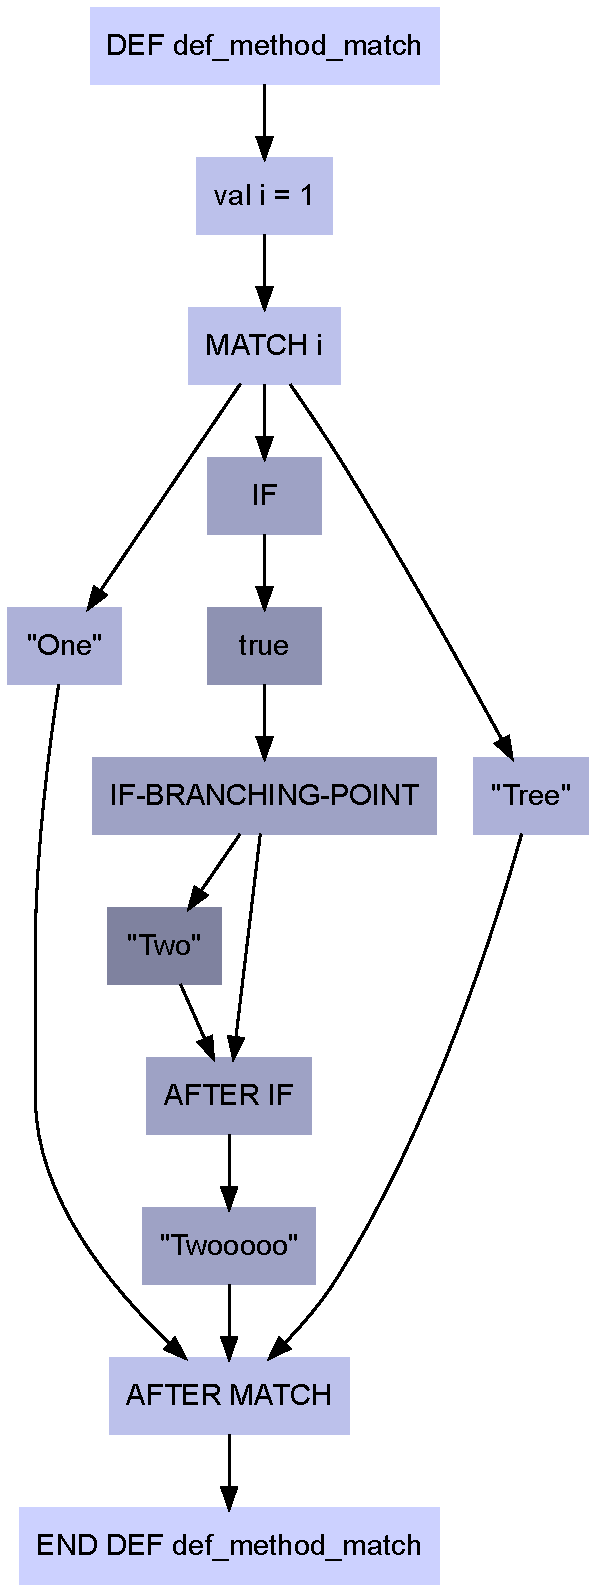
\includegraphics[width = 120pt]{fig/def_method_match.pdf}
  \caption{Control Flow Graph for the \code{def\_method\_match} method}
  \label{fig:def_method_match}
\end{figure}


\subsection{CC: Cyclomatic Complexity} \label{general_cc_explanation}
The notion of Cyclomatic Complexity is used to express the complexity of a function, based on its Control Flow Graph representation. It has been developed by McCabe \cite{mccabe1976complexity}. It is assumed that higher a Cyclomatic Complexity makes a program more fault prone \cite{basili1996validation}.
McCabe does this by representing the CFG in an adjacency matrix. The adjacency matrix is an $n x n$ matrix where each element $E_ij$ is 0 or 1, depending on whether there is an edge between node $i$ and $j$.

The method \code{def\_method\_match} from the previous section is now also shown in its adjacency matrix form in figure \ref{fig:adjacency_matrix}. In this thesis will prefer the graph from of the CFG.

\begin{figure}[H]
  \centering
  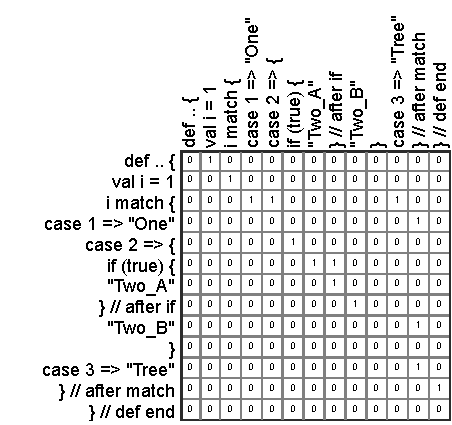
\includegraphics[width=300pt]{fig/adjacency_matrix.pdf}
  \caption{adjacency matrix for method def\_method\_match}
  \label{fig:adjacency_matrix}
\end{figure}


The formula to calculate the Cyclomatic Complexity of a CFG is as follows:
\[ CC = E - V + 2 * P \]
$E$ is the number of edges, $V$ the number of vertices, and $P$ the number of connected components. Where an connected component is a group of nodes, where each pair of nodes is connectable by series of edges. The CFG of \code{def\_method\_match} has 15 edges and 13 nodes, and thus is the Cyclomatic Complexity $15 - 13 + 2 * 1 = 4$


\subsection{Scalameta} \label{section_scalameta}
Scalameta is a library that can parse Scala code and stores its syntactic information in an easy to parse format. With this information, one can read the source code programmatically and calculate some properties out of it. A perfect tool to be used in this thesis. It is mainly developed by Eugene Burmako \cite{GithubScalametaContributers} and is now used at Twitter for building some of their tooling. Scalameta caches its syntactic data on disk in its own format. It could also have used the internal format of the compiler to store information in, but then the tool could break with future compiler updates.

To use Scalameta it can either be installed project specific by copying \code{Semanticdb.scala}\footnote{\url{https://gist.github.com/olafurpg/a74404dfee6b3da03892af17357074d9}} to the correct place in the project. Or it can be installed by copying this file to:\\ \code{~/.sbt/1.0/plugins/Semanticdb.scala}

We choose the latter, as it enables us to use Scalameta for many projects without needing to modify them. To build the required cache for Scalameta, invoke \code{SBT Semanticdb} from within the same folder as the \code{build.sbt} file.

If we take the code sample from figure \ref{fig:def_method_match_code} again, and pass it trough Scalameta, we will produce the AST shown in figure \ref{fig:def_method_match_AST}. For generating this simple example, the online tool "AST explorer"\footnote{\url{https://astexplorer.net/}} was used.

\begin{figure}[H]
  \centering
  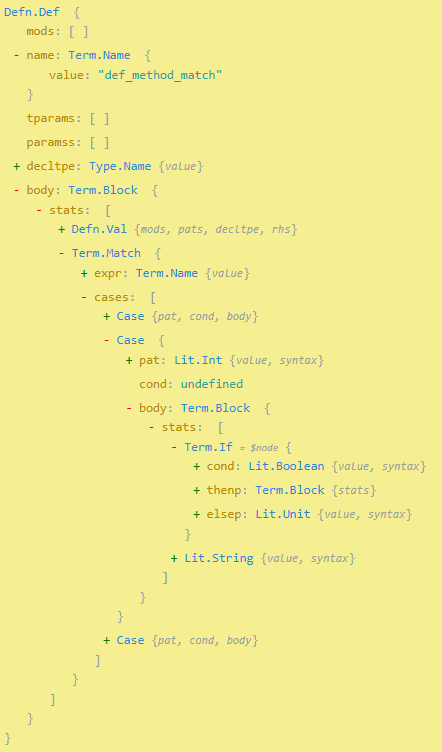
\includegraphics[width=220pt]{fig/def_method_match_AST.PNG}
  \caption{A screenshot of the AST generated with Scalameta.}
  \label{fig:def_method_match_AST}
\end{figure}


\subsection{Scalafix} \label{section_scalafix}
Scalafix is built upon Scalameta and adds semantic information to the data format. Every class, data member, method, ... gets a fully qualified name assigned to it. This fully qualified name is a string with all the necessary information to refer uniquely to an element in the project. This helps to reason about data types without having any ambiguity between types with the same name, but in a different name space.

Some examples of elements with the fully qualified name that got assigned by Scalafix:
\begin{itemize}
    \item A package: \code{org/shotdraw/standard/}
    \item A class in a package: \code{org/shotdraw/standard/StandardDrawingView\#}
    \item A trait in a package" \code{org/shotdraw/framework/Drawing\#}
    \item A method in a class: \code{org/shotdraw/standard/StandardDrawingView\#insertFigures()}
    \item An object in a package: \code{org/shotdraw/contrib/PolygonFigure.}
\end{itemize}

Types and methods are resolved and linked to each other. Using this information Scalafix can detect some semantic issues and propose corrections to them. For example, it can remove unused include statements, add braces around values that will be auto-tupled, convert the deprecated procedure and more \footnote{\url{https://scalacenter.github.io/scalafix/docs/rules/overview.html}}. We will however not use these correction features and only use the core functionality of Scalafix, which is to provide the semantic data.

The following code snippet illustrates how to use Scalafix to print the fully qualified name of classes in a file:
\begin{lstlisting}[language=scala]
  // Typical way to loop over the Scalameta AST:
  sdoc.tree.collect { 
    case defnClass: Defn.Class => {
      //               .symbol is Scalafix specific.
      println(defnClass.symbol.value)
    }
  }
\end{lstlisting}
When running the previous sample for the \code{StandardDrawingView.scala}\footnote{\url{https://github.com/EmileSonneveld/SHotDraw/blob/master/SHotDraw/src/main/scala/org/shotdraw/standard/StandardDrawingView.scala}} file, we get the following result: 
\begin{lstlisting}[language={}, basicstyle=\ttfamily\small]
org/shotdraw/standard/StandardDrawingView#
org/shotdraw/standard/StandardDrawingView#ASH#
org/shotdraw/standard/StandardDrawingView#DrawingViewMouseListener#
org/shotdraw/standard/StandardDrawingView#DrawingViewMouseMotionListener#
org/shotdraw/standard/StandardDrawingView#DrawingViewKeyListener#
\end{lstlisting}



\section{The overview pyramid} \label{section_the_overview_pyramid}
The overview pyramid gives a quick visual overview of the proportions of some characteristics of a project \cite{lanza2007objectOverviewPyramid}. The metrics it shows are described in chapter \ref{section_CalculatingTheMetrics}.
Some of those values are color graded depending on how they compare with other projects written in the same language. This color grading is described in chapter \ref{finding_common_values}.
Figure \ref{fig:pyramid_SHotDraw} shows an example of such an overview pyramid. The SHotDraw project will be described in section \ref{section_SHotDraw}. The overview pyramid is already implemented in multiple languages like PHP, Java and C++ \cite{Marek2010MetricsOOSoftware} \cite{Marinescu05iplasma}.

In this chapter, we will describe the overview pyramid for the Scala language, based on the book Object-Oriented Metrics in Practice \cite{lanza2007object}. First off, we will explain the abbreviations used in this pyramid. 

\begin{figure}[H]
  \centering
  \includesvg[width=\linewidth]{fig/pyramid_SHotDraw.svg}
  \caption{An overview pyramid of the Scala SHotDraw project, generated by Scalade.}
  \label{fig:pyramid_SHotDraw}
\end{figure}

\begin{itemize}
\item \textbf{The Size \& Complexity part}
The following metrics are related to the size and complexity of the code base. 
\begin{itemize}
    \item NOP: Number of packages. Discussion in section \ref{overview_pyramid_NOP}
    \item NOC: Number of classes. Discussion in section \ref{overview_pyramid_NOC}
    \item NOM: Number of operations. Discussion in section \ref{overview_pyramid_NOM}
    \item LOC: Lines of code. Number of packages. Discussion in section \ref{overview_pyramid_LOC}
    \item CYCLO: Cyclomatic number. Discussion in section \ref{overview_pyramid_CC}
\end{itemize}

\item \textbf{The Coupling part}
These metrics measure how strong the project is coupled. If there are many calls compared to the number of operations, the project is coupled intensively. If those calls often go to other classes, the system is very dispersed.
\begin{itemize}
    \item CALLS: Number of operation calls. Discussion in section \ref{overview_pyramid_CALLS}
    \item FANOUT: Number of called classes. Discussion in section \ref{overview_pyramid_FANOUT}
\end{itemize}

\item \textbf{The Inheritance part}
Here we will get to know how intensive object-oriented the system is.
\begin{itemize}
    \item ANDC: Average number of derived classes. Discussion in section \ref{overview_pyramid_ANDC}
    \item AHH: Average Hierarchy height. Discussion in section \ref{overview_pyramid_AHH}
\end{itemize}
\end{itemize}


\subsection{Calculating the metrics} \label{section_CalculatingTheMetrics}
All metrics are implemented using the data structures of Scalameta \ref{section_scalameta} and Scalafix \ref{section_scalafix}. First the semanticDb files are generated, then Scalafix loads this information and generates semantic information and then, we generate the calculate the metrics on this data. In section \ref{finding_common_values} we will explain what the threshold values are and how they are generated. Figure \ref{fig:architecture-overview_pyramid_pipeline} sums this up visually. In this chapter we will discuss what the metrics represent, how they were implemented, and how they differ to the Java implementation.

\begin{figure}[H]
  \centering
  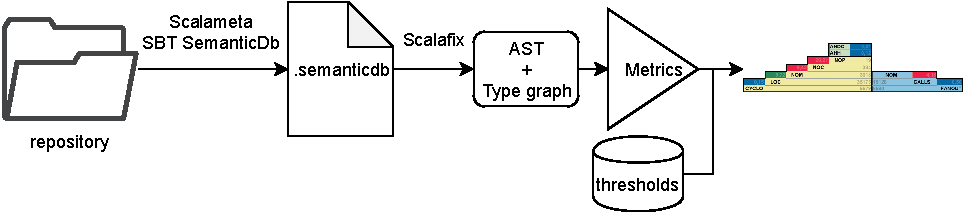
\includegraphics[width=300pt]{fig/architecture-overview_pyramid_pipeline.pdf}
  \caption{The pipeline of how Scalade parses a project to output the calculated metrics.}
  \label{fig:architecture-overview_pyramid_pipeline}
\end{figure}


\subsubsection{LOC: Lines of code} \label{overview_pyramid_LOC}
One of the simple metrics. Here all lines of code within all the method bodies in the project will be counted. Code outside methods, like import statements, fields, and so on don’t need to be counted in this version of LOC. In Scala, a class can also contain code outside of the methods. For the sake of simplicity, this is not counted. It is assumed that a higher LOC makes a program more fault prone. \cite{basili1996validation}. One study shows that LOC in a class is actually a good estimator of error-proneness \cite{GithubScalametaContributers}(Table 7.6).


\subsubsection{NOM: Number of operations} \label{overview_pyramid_NOM}
An operation is a piece of code that can be executed. In Java, an operation is always a method call. In Scala, methods that behave like they are an attribute also need to be counted, as they can also contain code.


\subsubsection{NOC: Number of classes} \label{overview_pyramid_NOC}
In Scala, there are more constructs than only classes.
\textbf{Trait}s are like classes, but cannot be instantiated. Classes and traits can also inherit from multiple traits.
An \textbf{Object} is like a class, but can only have one instance. This instance will be created the first time it is referenced. Unlike Traits and Classes, one cannot inherit from an object \cite{odersky2008programming}. \footnote{\url{https://docs.scala-lang.org/tour/singleton-objects.html}}
In Scala, Classes, Traits and Objects are all counted for this metric. Declarations in the same name space with the same name will be counted only once.

We will also count nested classes in this metric.


\subsubsection{NOP: Number of packages} \label{overview_pyramid_NOP}
In Java and Scala, packages help to break software systems into modules. A system with many packages could indicate that it is made by a very segregated developer group \cite{schroter2006if}.


\subsubsection{CYCLO: Cyclomatic complexity} \label{overview_pyramid_CC}
An overview of Cyclomatic Complexity was already given in section \ref{general_cc_explanation}. It is a way to express the complexity of a function based on the amount of control statements. This section will focus on its implementation.

We implemented the CC of a method by first creating the Control Flow Graph of a method and then counting the nodes and edges of this graph. The result is achieved by calculating $E - V + 2 * P$, where $E$ is the number of edges, $V$ the number of vertices and $P$, the number of connected components. $P$ will always be 1 in our case because we only evaluate one method at a time.

PMD implements CC by directly counting the branching control statements in the AST of a method\footnote{\url{https://github.com/pmd/pmd/blob/278bc2ab1b4bdec063a28e4baa4c7645b6a5eaea/pmd-java/src/main/java/net/sourceforge/pmd/lang/java/rule/design/StdCyclomaticComplexityRule.java}} This is an elegant way of solving this broblem, but we choose to go the traditional way with the CFG, because it allowed a better visual inspection of the workings of the algorithm, and thus manually verify its working. As an example, figure \ref{fig:def_method_match} shows the generated CFG for method for function. \code{def\_method\_match}.

The Scala language has some constructs that aren't present in Java. Special care has been made to handle the \code{match} statement correctly, \code{continue} statements are not implemented in Scala and so didn't need to be implemented. If-statements that are used as ternary operators will not make a splitting point in the graph. These are rare enough to not have a significant influence on the total CC. Inline functions are ignored. If taken into account their CC should be multiplied by the amount of times the function is called and then added to the parent function CC. 


\subsubsection{CALLS: Number of operation calls} \label{overview_pyramid_CALLS}
As in \ref{overview_pyramid_NOM}: An operation is a piece of code that can be executed. In Java, an operation is always a method call. In Scala, properties also need to me counted, as they can also contain code.

CALLS gives an indication of how many times any operation is called in the project. If the same method is called multiple times within one method body, it will only be counted once.


\subsubsection{FANOUT: Number of called classes} \label{overview_pyramid_FANOUT}
This metric is calculated summing the FANOUT metric for each operation in the project. The FANOUT metric says something of the body of an operation. It specifies on how many different classes this operation calls methods on. For example the method in code sample \ref{fig:FanoutTest} will have a FANOUT of 2. \code{.x} and \code{.y} both are from the \code{Point class} and will only count once. \code{.prettyPrint()} is from a different class, namely \code{Vector} and will increase the FANOUT with 1.

According to the book, this gives an idea of how dispersed the operations in the project are. \cite{lanza2007object}.

\begin{figure}[H]
    \centering
    \begin{lstlisting}[language=scala]
  def FanoutTest(point: Point): Vector = {
    var vec:Vector = makeVector(point.x, point.y)
    println(vec.prettyPrint())
    vec
  }
    \end{lstlisting}
    \caption{The method FanoutTest has a FANOUT of 2}
    \label{fig:FanoutTest}
\end{figure}


\subsubsection{ANDC: Average number of derived classes} \label{overview_pyramid_ANDC}
This metric will count the amount of direct child classes/traits/objects that a certain class/trait has. Only direct children will be counted, children of children will not influence this metric. This metric gives an idea of the width of a hierarchy tree.

Implementation wise, an extra step is implemented before calculating ANDC. For each class, Scalafix only exposes the parent classes, not the child classes. The type graph is first rebuilt so that each class also knows its child classes. We then simply go over all classes, count their children and divide by the number of classes.


\subsubsection{AHH: Average Hierarchy height} \label{overview_pyramid_AHH}
AHH is calculated by computing the average of the hierarchy height of each 'family' of classes. A family is a cluster of classes where each pair of classes can be connected with a path of 'inherits from' and 'is inherited from' relations. Figure \ref{fig:AHH-families} illustrates how classes could be divided in such families. Interfaces are not part of the type hierarchy. However, interfaces don't exist in Scala, instead, they are implemented with traits. Distinguishing if a trait should be categorized as a class or an interface is a subjective decision, instead of making the difference, we will categorize all traits like classes, and count them in the hierarchy. AHH gives us an idea of the height of the hierarchy structure. A project with a very high AHH could mean that a change to one class could have a propagating effect to many child classes. 

\begin{figure}[H]
  \centering
  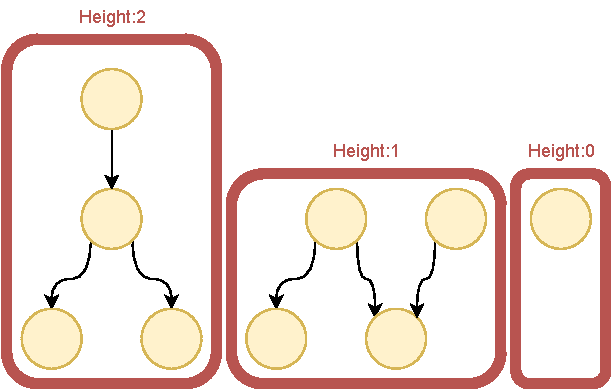
\includegraphics[width=200pt]{fig/AHH-families.pdf}
  \caption{Families indicated in red, with their hierarchy height}
  \label{fig:AHH-families}
\end{figure}

The middle family with height 1 contains a class with multiple parents. This is because, unlike Java, Scala can use traits and a class can inherit from multiple traits. In Scala, traits can be used as a class or as an interface. An interface-trait is just a trait with only abstract functions. We take the naive approach and treat every trait like a class.\footnote{We could also treat a trait like an interface if it does not implement any methods. And interfaces can be avoided in the calculation.} Our algorithm to calculate the hierarchy height will be slightly more complex than in Java. 

\textbf{In Java}, it suffices to take a node without parents to know it is at the top of a hierarchy. After that once can recursively loop all children and find the deepest one.

\textbf{In Scala}, the type hierarchy is actually a directed acyclic graph, so we will use graph traversal. We will start the algorithm at an arbitrary node and loop the family graph with depth-first traversal, marking visited nodes to avoid infinite loops. While traversing, the current depth will be remembered. This current depth will start at 0, increases when jumping to a child, and decreases when jumping to a parent. Note that the depth can be negative. At the end of the traversal, we can calculate the hierarchy height by taking the difference between the highest and the lowest depth. 

The following paragraph explains the Scala algorithm in pseudo code, accompanied with figure \ref{fig:AHH-height} to show this visually.

\begin{lstlisting}[language=R]
function getAHH(typeGraph):

    # symbolNodes is a list of all 
    # project specific classes and traits.
    for node in symbolNodes: 
        node.clusterId = -1

    function infectClusterWithId(node, id):
        [recursevly walk all parent and child relationships and do]:
            node.clusterId = id

    clusterStarters = [empty list of nodes]
    currentClusterId = 0
    for node in symbolNodes:
        if node.clusterId < 0: # skip nodes already in a cluster
            currentClusterId += 1
            infectClusterWithId(node, currentClusterId)
            clusterStarters += node

    heightList = [empty list of ints]
    for clusterStarter in clusterStarters:
        minOffset = 0
        maxOffset = 0

        function searchExtremeOffsets(currentNode, currentOffset):
            [update min and max offset based on currentOffset]

            for child in node.children:
                searchExtremeOffsets(child, currentOffset + 1)

            for child in node.parent:
                searchExtremeOffsets(child, currentOffset - 1)

        searchExtremeOffsets(clusterStarter, 0)
        heightList += maxOffset - minOffset
    return average(heightList)
\end{lstlisting}

\begin{figure}[H]
  \centering
  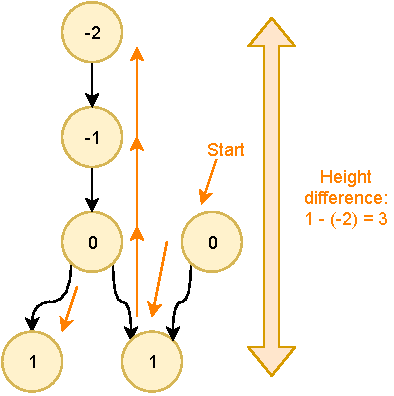
\includegraphics[width=200pt]{fig/AHH-height.pdf}
  \caption{Example of how the algorithm traverses a family graph to calculate the hierarchy height.}
  \label{fig:AHH-height}
\end{figure}


\subsection{Selecting common values for the Overview Pyramid} \label{finding_common_values}
The overview pyramid displays a many values and some ratios between them. Developers don’t always have an intuition of what values are good and what are bad. This is solved by giving a color scale to some of the values. Values indicated in red would be higher than normal, blue lower than normal and green, normal. In the size part, red could indicate classes with many methods, methods with many lines of code and so on. Blue would indicate the contrary. Both cases would tell us that something is off and often they go hand in hand. For example, when there are many methods per class (red), chances are high that these methods will be very large to accommodate all the logic. Only the ratios between metrics and the inheritance metrics are color graded. The raw size values are not color graded, as is wouldn't give insight in the programming style in the project, but only show the size of the project. The inheritance metrics also stay stable between projects between different size, and so these raw metrics can be color graded too.

In this section, we will analyze 241 Scala projects to determine what the common values for the ratios and the inheritance metrics are. Based on these values, we will determine thresholds that will decide in what color a value should be displayed.

We can then color the numbers as follows:
\begin{itemize}
    \item \textbf{Blue:} If the value is lower than the mean, minus one standard deviation
    \item \textbf{Green:} By default
    \item \textbf{Red:} If the value is higher than the mean, plus one standard deviation
\end{itemize}

This is illustrated in figure: \ref{fig:Standard_deviation_diagram}.
\begin{figure}[H]
  \centering
  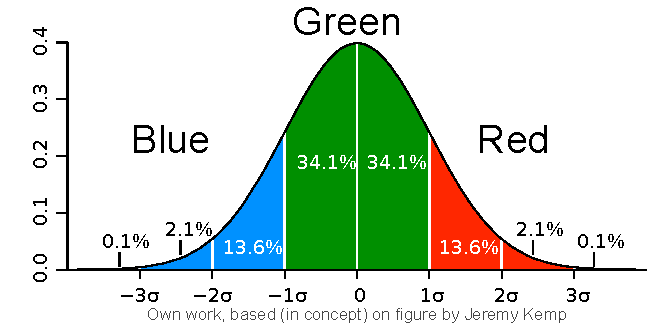
\includegraphics[width=200pt]{fig/Standard_deviation_diagram.pdf}
  \caption{Choice of color based on location in the distribution}
  \label{fig:Standard_deviation_diagram}
\end{figure}


\subsubsection{Running the large scale analysis} \label{running_large_scala_analysis}
A large set of Scala projects was obtained as follows:
\begin{enumerate}
    \item Using the GitHub API\footnote{https://developer.github.com/v3/search/legacy/\#search-repositories}, many projects with available source code were listed. The first ~900 projects with most stars when searching for the 'Scala' keyword were downloaded.
    \item Out of all these results a list was composed by selecting all the values for "URL" out of the returned JSONs. This list contained 862 URLs.
    \item Each URL was then cloned to a local computer by running "git clone <URL>" for every URL.
    \item 'sbt semanticdb' was executed on each cloned repository. The projects that did not compile in this step were removed. To maximize the amount of projects that do compile, the following settings were changed\footnote{Complete implementation: \url{https://gitlab.soft.vub.ac.be/maproef1819-emile/maproef1819-emile/blob/master/thesisScalaProject/src/main/scala/Cmd.scala\#L95}}:
    \begin{itemize}
        \item Java 8 was chosen, as SBT could compile more programs under Java 8 than Java 11.
        \item The JVM was given more RAM.
        \item SBT's whole program hierarchy had to be killed after a failure; otherwise future builds would run out of memory.
    \end{itemize}
    This resulted in 296 successful builds.
    \item The Scala implementation of the overview pyramid was then ran on all these projects. Projects with less than 500LOC where filtered away.
    This reduced the number of projects further to 241. On these projects, the metrics for the overview pyramid were calculated, and the results stored in a database.
\end{enumerate}


\subsubsection{Analysing the data}
After the metrics of the 241 projects were collected, the results could be analyzed. To find good threshold values, the technique relies on the idea that the values are normally distributed, that is why we first need to verify if this is the case. 


As seen in figure~\ref{fig:all_plots_scala}, almost all metrics follow a skewed bell curve, so we can use the concept of standard deviation and mean. Every graph also displays the value for z-score -1 and for z-score +1\footnote{Statistical calculations where done with python and matplotlib.}. These values will be used as thresholds in the overview pyramid. For example, if a pyramid has an ANDC value under 0.63, it will be displayed in blue.
\begin{figure}[H]
    \centering
    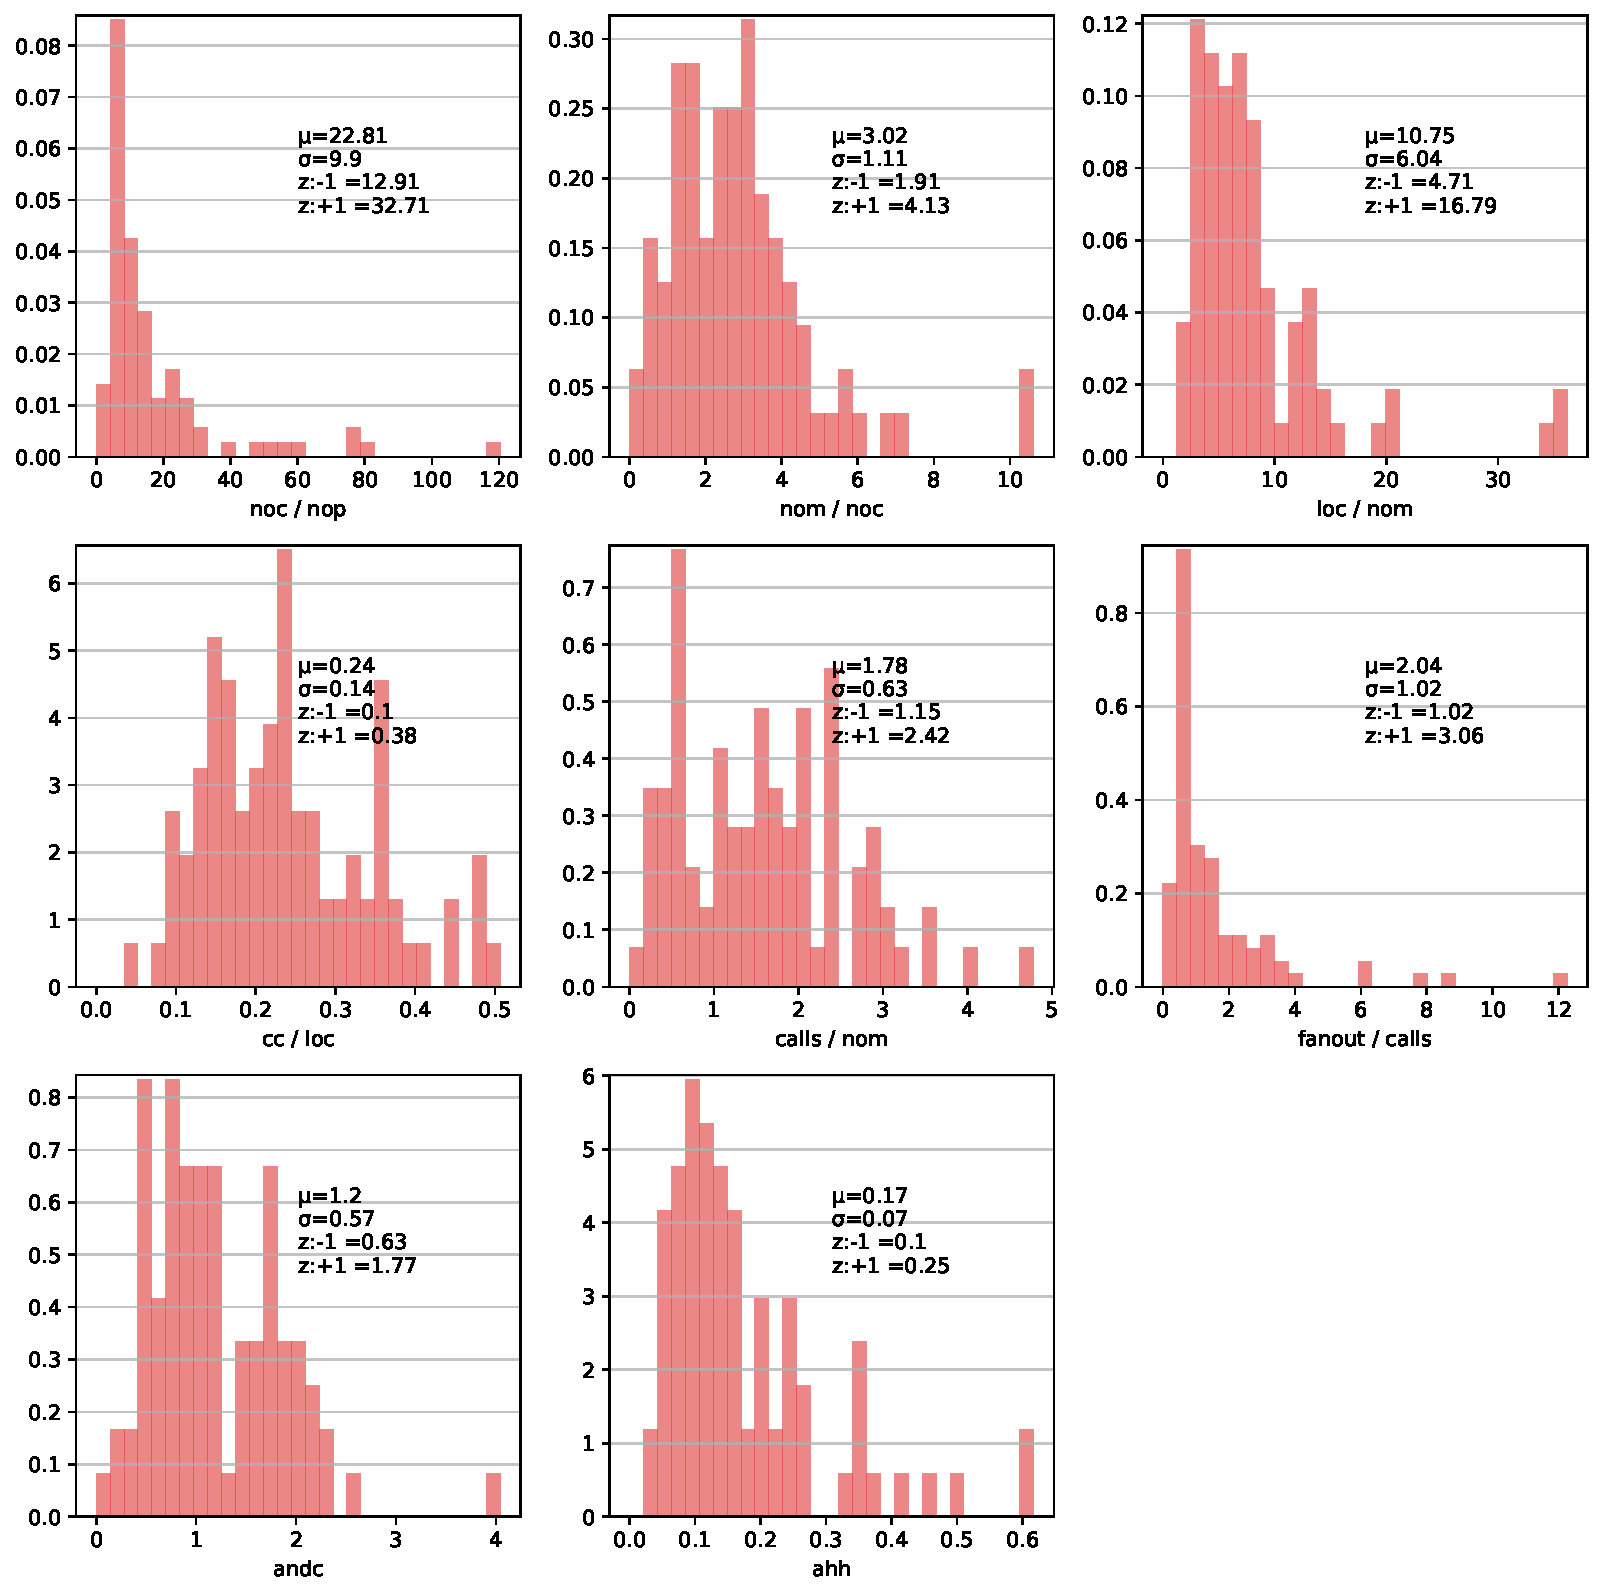
\includegraphics[width=\textwidth]{fig/hist_ratios/all_plots_scala.pdf}
    \caption{Distributions of all metrics in the Scala overview pyramid}
    \label{fig:all_plots_scala}
\end{figure}

\section{Detecting code smells} \label{section_detecting_code_smells}
Research tells us that it is considered good practice to refactor code often and that code smells are a good way to detect places that should be refactored first \cite{mantyla2003taxonomy}.
Some research has been done to detect code smells in software projects \cite{van2002java}. These can indicate poorly structured code and an opportunity to refactor them to enhance the code base.
We will describe some common metrics used to find those smells and then we will describe the smells themselves. Trough the examples, we will also use the SHotDraw project to illustrate some cases. Figure \ref{fig:architecture-code_smells_pipeline} gives a brief overview of the architecture for detecting code smells. New design smells can be implemented in the \code{MeasureProject} object in Scalade.

\begin{figure}[H]
  \centering
  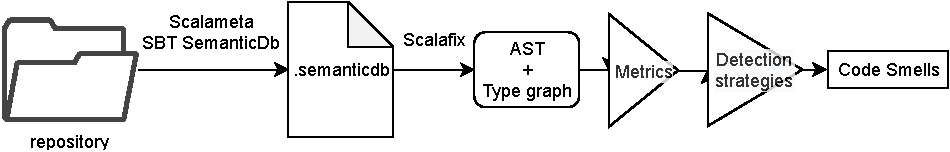
\includegraphics[width=300pt]{fig/architecture-code_smells_pipeline.pdf}
  \caption{Detecting code smells pipeline.}
  \label{fig:architecture-code_smells_pipeline}
\end{figure}

\subsection{Example project: JHotDraw / SHotDraw} \label{section_SHotDraw}
In this thesis, we will use JHotDraw and SHotDraw to evaluate our metrics.
JHotDraw is a small open source project implemented in Java\footnote{\url{https://sourceforge.net/projects/jhotdraw/}}. It is used in some research papers \cite{barkmann2009quantitative} \cite{marin2007integrated}. It has also been transpired to a Scala project named SHotDraw\footnote{\url{https://github.com/EmileSonneveld/SHotDraw/tree/master/SHotDraw}}.
Having the same project implemented in 2 languages makes it easy to compare Java tools against our Scala tools.


\subsection{Metrics}
Before describing the code smells them self, we will first discuss the metrics used. Like the with the chapter for the overview pyramid, some details will be implemented differently than in the Java language for example. 

\subsubsection{ATFD: Access to Foreign Data} \label{metric_ATFD}
Methods in a class mostly access properties inside its own class. But sometimes, against any good practice, properties from other classes are accessed. Those are considered as access to foreign data. ATFD will count all those cases.

Our version of ATFD is implemented to stay close to that of PMD. However, a bug was discovered in PMD which made it difficult to align both implementations. A bug report was submitted and fixed within 2 weeks\footnote{\url{https://github.com/pmd/pmd/issues/1910}}. This made it easier to get both implementations in line. 
In Java, getters and setters are normal methods; they however indicate almost direct access to a field and are counted as such. To check weather a method is a getter or a setter, PMD checks the prefix of the method. If it starts with 'get', 'set', or 'is', the method will be counted as an attribute access. The same logic has been implemented in the Scala version. As an extra, Scala can also explicitly define getters and setters\footnote{\url{https://www.dustinmartin.net/getters-and-setters-in-scala/}}. The following fragment illustrates that using 
\begin{lstlisting}[language=scala]
class Person() {
 private var _age = 0
 def age = _age  // Getter
 def age_= (value:Int):Unit = _age = value // Setter
}
\end{lstlisting}


\subsubsection{WMC: Weighted Method Count} \label{metric_WMC}
This metric that sums the Cyclomatic Complexity of all operations in a class. Giving a measure of how complex the class is.


\subsubsection{TCC: Tight Class Cohesion} \label{metric_TCC}
Considering all method pairs. Method pairs that use a common property are linked, all others not. TCC is now the result of dividing the linked method pairs by the total amount of method pairs.

TCC is a good metric to test class cohesion. A class with 2 separate functionalities will have 2 clusters of methods that are not linked to each other, resulting in a low cohesion. A cross cutting concern could however artificially increase the cohesion. For example, if a large class has a logger object saved in a property, and many methods use this property, the class will have an artificially high cohesion.


\subsubsection{LAA: Locality of Attribute Accesses} \label{metric_LAA}
This is a metric for a method. It can easily be calculated with the following formula:
\[\frac{\#\:own\;attributes\;accessed}{\#\:total\;attributes\;accessed} \]


\subsubsection{FDP: Foreign Data Providers} \label{metric_FDP}
Indicates the number of unique classes from which attributes are accessed, excluding the current class of course.


\subsubsection{MAXNESTING: Maximum Nesting Level} \label{metric_MAXNESTING}
MAXNESTING indicates how many control structures deep a method goes. A method with 4 nested if-statements will have a MAXNESTING value of 4. A method with 4 if-statements next to each other will have a MAXNESTING of 1.

This metric could have been implemented going on the Control Flow Graph with depth first traversal. Each time a node that has multiple outgoing branches is passed, a counter increases, each time a stack frame is unwinded, a counter decreases. MAXNESTING would then be the maximum value the counter had during the recursion.

However, this time we will not use the CFG, instead, we will recursively loop over the AST of the method. We will recurse into any construct we find on the way, even though it is not a control structure. Also, here we will keep a counter that tracks the current depth. Each time we recurse into a control structure, the counter increases, each time we go out of a control structure, the counter decreases. The maximum value the counter had during the recursion will be the MAXNESTING of this method.


\subsubsection{NOAV: Number Of Accessed Variables} \label{metric_NOAV}
Counts all variables accessible in the scope of a method. Including, but not limited to: local variables, method parameters, class attributes and global variables.

If a method has a higher NOAV than a human can keep in his short-term memory (5-7 items), then this method will be very difficult to reason with.


\subsection{The Code Smells}
A design smell can be detected with a \textit{detection strategy}. A detection strategy is an expression with conditions and logical operators. If the expression evaluates to $True$, the strategy detected a design smell. For example, the GodClass detection strategy measures 3 metrics for a class, compares each metric with a certain value, and combines those 3 comparisons with an $And$ operator. Only if the 3 comparisons return $True$, then the strategy will detect the smell it was designed for.

Those detection strategies can use vague words like "few" or "several". For practical purposes, we will use a number between 2 and 5 when terms like 'FEW' and 'SEVERAL' are used, as shown in figure \ref{fig:semantic_values}.

\begin{figure}[H]
    \centering
    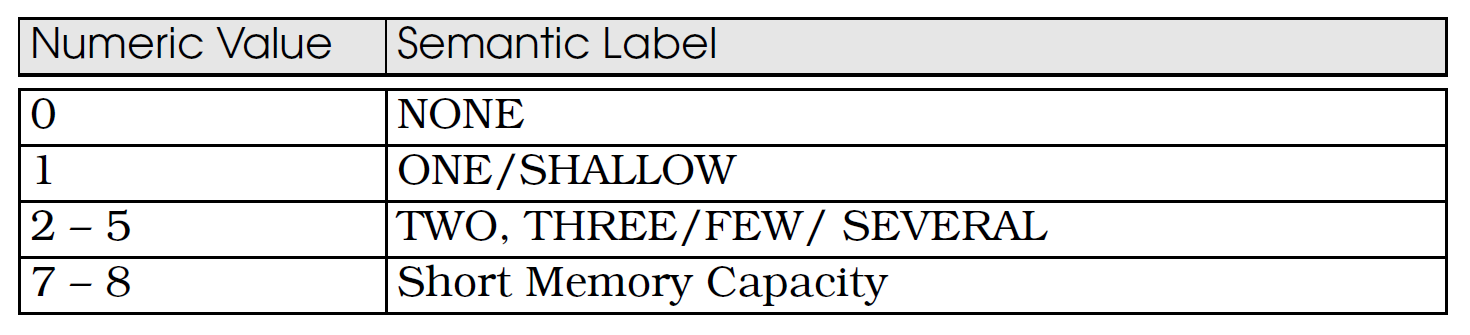
\includegraphics[width=200pt]{fig/semantic_values.PNG}
    \caption{Threshold values associable with generally accepted semantics from \protect\cite{lanza2007object}}
    \label{fig:semantic_values}
\end{figure}

In this chapter we will discuss and implement 3 detection strategies: \textbf{GodClass}, \textbf{FeatureEnvy} and \textbf{BrainMethod}. For each detection strategy, we explain how it works, apply it on the SHotDraw project and study one of the detected instances of the smell. We will also compare with the implementation in PMD where relevant. We ran Scalade on 241 projects to detect design smells 45 of them exhibited design smells, totaling 45 cases of GodClass, 155 cases of FeatureEnvy and 11 cases of BrainMethod. Full list of findings can be found in appendix \ref{appendix_design_smells_in_sample_projects}. 


\subsubsection{God class}
In a healthy system, functionality is separated in multiple classes. In a GodClass, this is not the case. A GodClass pulls too much functionality to itself making it difficult to test, reason about and refactor. Each change to a GodClass can potentially have effect on many features residing in the same class. Refactoring however is probably worthwhile\cite{du2006does}.
Scalade can detect GodClasses in Scala projects. We do this by calculating 3 metrics on each class and when they pass certain thresholds, our detection strategy indicates that it is a GodClass.

\begin{figure}[H]
    \centering
    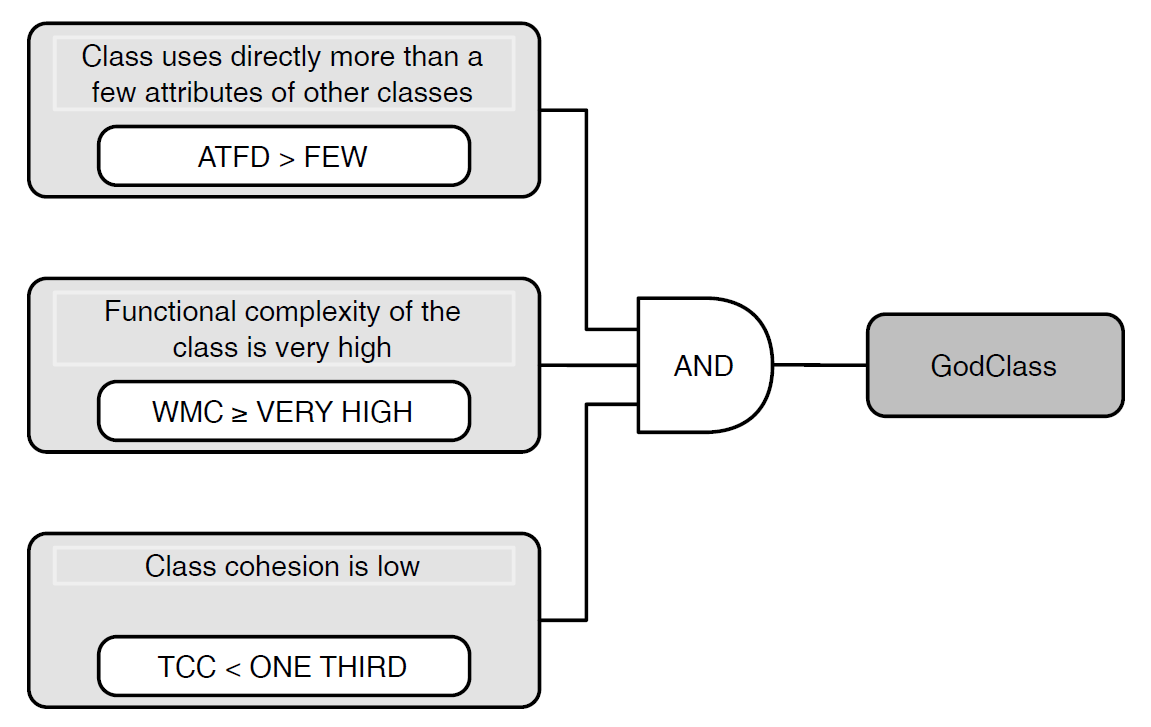
\includegraphics[width=200pt]{fig/lanza_GodClass.PNG}
    \caption{The GodClass detection strategy from \protect\cite{lanza2007object}}
    \label{fig:lanza_GodClass}
\end{figure}

The exact thresholds are based on the table in \cite{lanza2007object}(Page 18) and the implementation of PMD:
% C:\Users\emill\dev\maproef1819-emile\thesisScalaProject\src\main\scala\MeasureProject.scala
\begin{itemize}
    \item $ATFD > 2$
    \item $WMC >= 47$ where 47 is taken from the PMD project.
    \item $TCC < 1/3$
\end{itemize}

ATFD is described in section \ref{metric_ATFD}, WMC in \ref{metric_WMC}, TCC in \ref{metric_TCC}.

In the SHotDraw project, we found the following GodClass smells:
\begin{itemize}
    \item org/shotdraw/application/DrawApplication\#
    \item org/shotdraw/figures/LineConnection\#
    \item org/shotdraw/figures/TextFigure\#
    \item org/shotdraw/standard/CompositeFigure\#
    \item org/shotdraw/standard/ConnectionTool\#
    \item org/shotdraw/standard/StandardDrawingView\#
    \item org/shotdraw/util/Bounds\#
\end{itemize}

Let us consider \code{StandardDrawingView}\footnote{\url{https://github.com/EmileSonneveld/SHotDraw/blob/832b256a241d857ff9775eac3264d468059f56f9/SHotDraw/src/main/scala/org/shotdraw/standard/StandardDrawingView.scala}} as an example. It has the following properties: ATFD=45, WMC=156, TCC= 0.044 and thus is detected as GodClass.

It is a class responsible for showing an interface to the end user, and dispatching its keyboard and mouse inputs to the user selected tool, so that this tool can edit the \code{Drawing}. This is a lot of responsibilities, but it is is difficult to split the class much further. One method in this class has FeatureEnvy and should be refactored; this will be discussed in the following section.

Let's consider a false positive: \code{TextFigure}. With ATFD=37, TCC=0.11, WMC=53 it is classified as a GodClass while it feels quite structured. It only contains the necessary complexity for moving the figure, drawing the text and serialization. The class could be split in pieces, but this would only increase complexity. We would not recommend refactoring this class; however, this smell is still a good indication that this is a complex class and a developer should be cautious when making edits.

\subsubsection{Feature Envy}
Feature Envy occurs when a method calls many attributes and operations of another class. This could mean that the method is implemented in the wrong place and should be moved to another class. This design smell is simple to refactor away, unlike the GodClass.
Feature envy is detected by taking 3 metrics on each method and feeding this to the detection strategy, described in figure \ref{fig:lanza_FeatureEnvy}.

\begin{figure}[H]
    \centering
    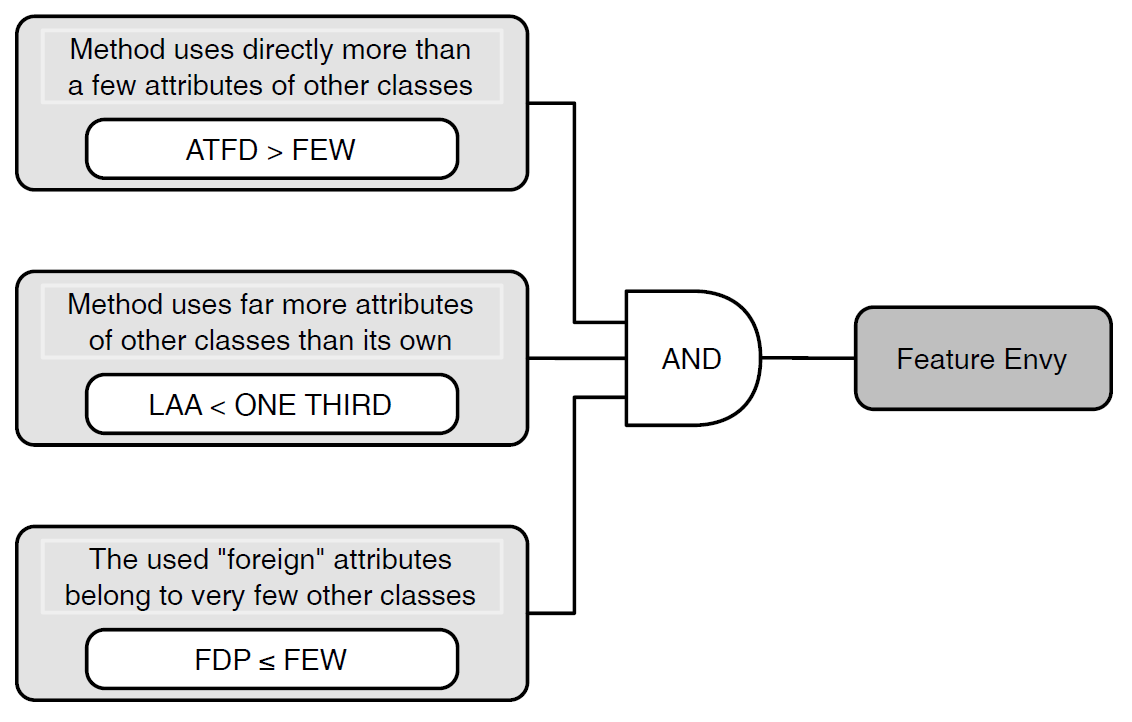
\includegraphics[width=200pt]{fig/lanza_FeatureEnvy.PNG}
    \caption{The Feature Envy detection strategy from \protect\cite{lanza2007object}}
    \label{fig:lanza_FeatureEnvy}
\end{figure}

For the $FEW$ value we choose 4.)
\begin{itemize}
    \item $ATFD > 4$
    \item $FDP <= 4$
\end{itemize}

ATFD is described in section \ref{metric_ATFD}, LAA in \ref{metric_LAA}, FDP in \ref{metric_FDP}.

In the SHotDraw project, we found the following methods with Feature Envy:
\begin{itemize}
    \item org/shotdraw/standard/StandardDrawingView\#insertFigures().
    \item org/shotdraw/util/RedoCommand\#execute().
    \item org/shotdraw/util/UndoCommand\#execute().
\end{itemize}

Consider $StandardDrawingView\#insertFigures()$ as an example. It has the following properties: ATFD=5, LAA=0.16 FDP=4 and thus is detected to have FeatureEnvy.

Most of the methods in $StandardDrawingView$ interact with Java AWT and the $Drawing$ object. However, the $insertFigures$ method uses domain-specific knowledge that the class $StandardDrawingView$ should not know about. It interacts with $Drawing$, $ConnectionFigure$ and $Figure$ at the same time. The method could be moved inside under the $Drawing$ trait or under the $Figure$ trait to enhance separation of concerns.

\begin{lstlisting}[language=scala]
/**
   * Inserts a Seq[Figure] of figures and translates them by the
   * given offset. This function is used to insert figures from clipboards (cut/copy)
   *
   * @return enumeration which has been added to the drawing. The figures in the enumeration
   *         can have changed during adding them (e.g. they could have been decorated).
   */
  def insertFigures(fe: Seq[Figure], dx: Int, dy: Int, bCheck: Boolean): Seq[Figure] = {
    if (fe == null) {
      return Seq[Figure]()
    }

    var vCF = ArrayBuffer[ConnectionFigure]()
    val visitor = new InsertIntoDrawingVisitor(drawing)
    fe foreach (f => f match {
      case cf: ConnectionFigure => vCF += cf
      case _ if f != null => 
        f.moveBy(dx, dy)
        f.visit(visitor)
    })
    vCF foreach { cf =>
      val sf = cf.startFigure
      val ef = cf.endFigure
      if (figureExists(sf, drawing.figures) && figureExists(ef, drawing.figures) && (!bCheck || cf.canConnect(sf, ef))) {
        if (bCheck) {
          val sp = sf.center
          val ep = ef.center
          val fStartConnector = cf.startFigure.connectorAt(ep.x, ep.y)
          val fEndConnector = cf.endFigure.connectorAt(sp.x, sp.y)
          if (fEndConnector != null && fStartConnector != null) {
            cf.connectStart(fStartConnector)
            cf.connectEnd(fEndConnector)
            cf.updateConnection()
          }
        }
        cf.visit(visitor)
      }
    }
    this.addToSelectionAll(visitor.getInsertedFigures)
    return visitor.getInsertedFigures
  }
\end{lstlisting}


\subsubsection{Brain method}
A method which is so large that it becomes difficult to reason about is called a brain method. A brain method indicates that functionality is not spread well across methods in a class. Like a GodClass, a brain method is difficult to refactor. Isolating pieces of the method in different smaller methods could prove challenging, as for each change, many features of this large method could break, and bugs could be introduced.

\begin{figure}[H]
    \centering
    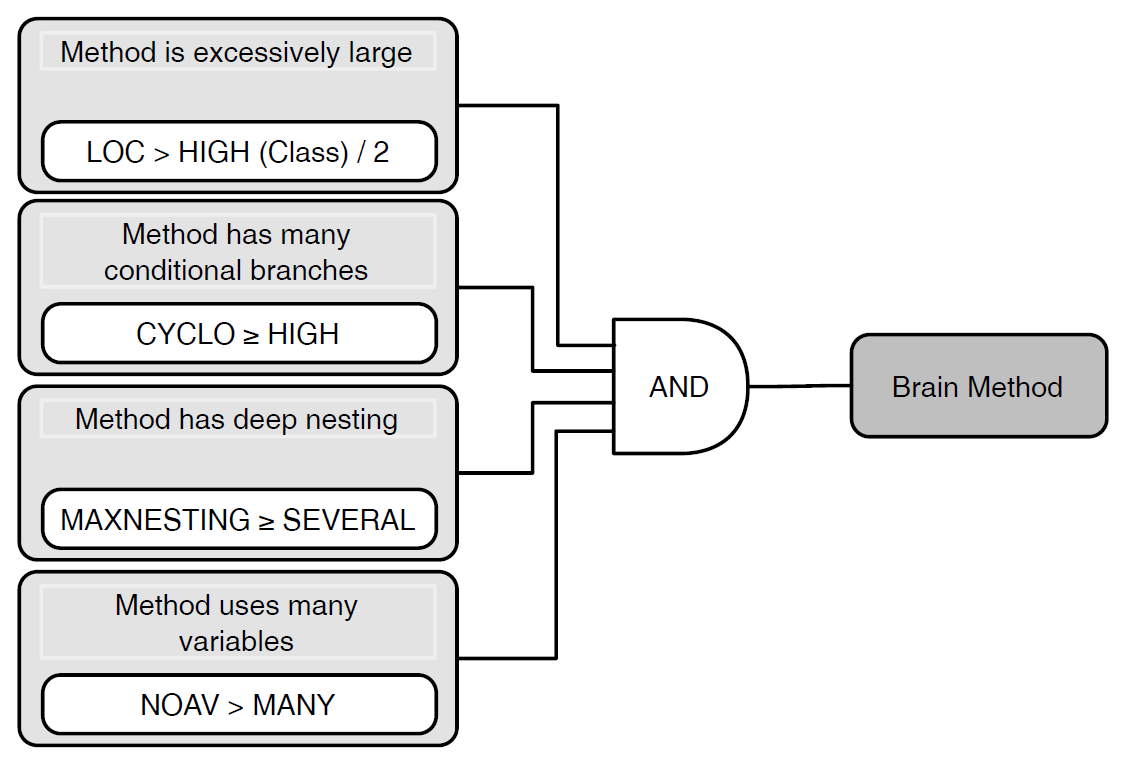
\includegraphics[width=200pt]{fig/lanza_BrainMethod.PNG}
    \caption{The Brain Method detection strategy from \protect\cite{lanza2007object}}
    \label{fig:lanza_BrainMethod}
\end{figure}

\begin{itemize}
    \item $CYCLO > 10$
    \item $MAXNESTING > 3$
    \item $NOAV > 3$
\end{itemize}
LOC is the number of code lines in the methods, CYCLO is the Cyclomatic Complexity of the method, LAA is described in \ref{metric_LAA}, MAXNESTING in \ref{metric_MAXNESTING}.

In the SHotDraw project, we found only one brain method:
\begin{itemize}
    \item org/shotdraw/contrib/dnd/JHDDropTargetListener\#drop().
\end{itemize}

$drop$ has the following properties: LOC= 81, CYCLO= 12, MAXNESTING= 5, NOAV= 13. In a Trait that only has 122 LOC, this is considered a BrainMethod. And indeed, when reading the method, we see that it is very complicated, a big if-else case with 4 branches fills the function. The if-statements always test on type, this could normally be converted into polymorphism of a visitor pattern, but the $DropTargetDropEvent$ object is defined and created in an external library, this is not possible. As a last resort, the method could still be separated in multiple smaller methods.

\begin{lstlisting}[language=scala, basicstyle=\ttfamily\small]
  /**
   * The drag operation has terminated with a drop on this DropTarget.
   * Be nice to somehow incorporate FigureTransferCommand here.
   */
  def drop(dtde: DropTargetDropEvent) {
    System.out.println("DropTargetDropEvent-drop")
    if (dtde.isDataFlavorSupported(DNDFiguresTransferable.
      DNDFiguresFlavor) == true) {
      log("DNDFiguresFlavor")
      if ((dtde.getDropAction & DnDConstants.ACTION_COPY_OR_MOVE) != 0) {
        log("copy or move")
        if (dtde.isLocalTransfer == false) {
          System.err.println("Intra-JVM Transfers not implemented for figures yet.")
          dtde.rejectDrop
          return
        }
        dtde.acceptDrop(dtde.getDropAction)
        // ... for the sake of brevity, some code is left away ...
      } else {
        dtde.rejectDrop
      }
    } else if (dtde.isDataFlavorSupported(DataFlavor.stringFlavor)) {
      log("String flavor dropped.")
      dtde.acceptDrop(dtde.getDropAction)
      val o = DNDHelper.processReceivedData(DataFlavor.stringFlavor, dtde.getTransferable)
      if (o != null) {
        log("Received string flavored data.")
        dtde.getDropTargetContext.dropComplete(true)
      }
      else {
        dtde.getDropTargetContext.dropComplete(false)
      }
    }
    else if (dtde.isDataFlavorSupported(DNDHelper.ASCIIFlavor) == true) {
      log("ASCII Flavor dropped.")
      // ... for the sake of brevity, some code is left away ...
    }
    else if (dtde.isDataFlavorSupported(DataFlavor.javaFileListFlavor)) {
      log("Java File List Flavor dropped.")
      // ... for the sake of brevity, some code is left away ...
    }
    fLastX = 0
    fLastY = 0
  }
\end{lstlisting}


\section{Evaluation} \label{section_evaluation}
To recap, we developed the tool Scalade, that has the functional capabilities of iPlasma and PMD. In this chapter, we will evaluate the results of this tool against the original versions. Figure \ref{fig:architecture-overview} will help to explain what we will test in this chapter. On the top half, we see Scalada, the tool that we implemented, on the bottom half, we see iPlasma and PMD. On both sides, a large sample of projects from GitHub where selected int their respective language. Scalade will parse the Scala projects (using Scalameta and Scalafix) and will output a series of overview pyramids. IPlasma will Parse the Java projects and output some overview pyramids. Both implementations of the overview pyramid use a set of thresholds to indicate in what color certain values should be shown. For iPlasma, it is unknown on what projects those thresholds are based. For Scalade, the list of projects can be found in appendix \ref{appendix_list_of_analyzed_projects}


\begin{figure}[H]
  \centering
  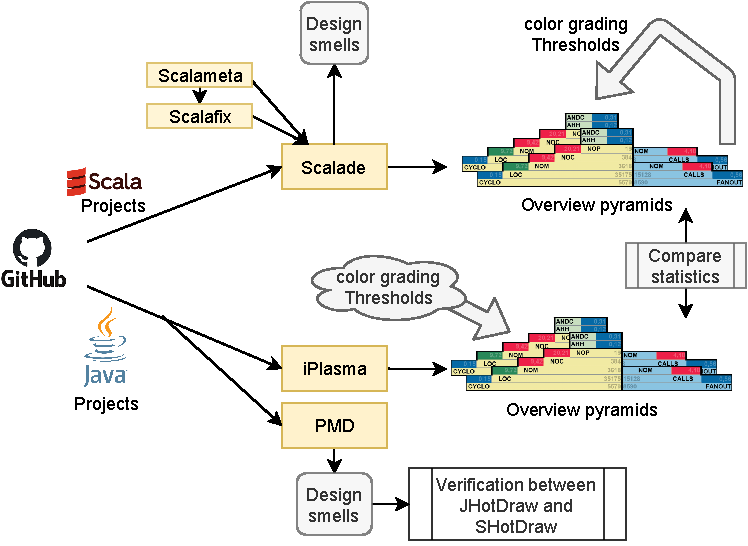
\includegraphics[width=300pt]{fig/architecture-overview.pdf}
  \caption{Architecture}
  \label{fig:architecture-overview}
\end{figure}





\subsection{Qualitative comparison between overview pyramid from iPlasma vs Scalade} \label{section_compare_pyramids}
The code between JHotDraw and SHotDraw is on high and low level equivalent. The language differs, but the constructs look a lot like each other. This means that the overview pyramids should show equivalent results. In this section we will compare those 2 pyramids. 

Figure \ref{fig:JHotDraw_iPlasma} illustrates the overview pyramid for the JHotDraw project. And \ref{fig:pyramid_SHotDraw_Again} show the overview pyramid for the project again. Both show the same colors at the "Size and Complexity" side. It seems like the developer wrote many methods per class, with very few lines of code per methods, but a relatively high cyclomatic complexity. At the top of the pyramid, iPlasma used an unknown metric called "NDD". Upon decompilation, it seems that this stands for "Number of Children for model classes" we assume that is the same metric as ANDC, an indeed, the Java and Scala implementation to compare. Further, in the "Inheritance" part, AHH or HIT shows a slightly different value, but both end up as red. This is indeed a very high value. This could be due the many cross cutting concerns that are implemented as \code{Storable}, \code{Undoable} and \code{Command} those are in both of the implementations residing at the top of huge type hierarchies. The CALLS/NOM ratio is indicated in blue for Java and Green for Scala. For FANOUT/CALLS the results are even more different, the ratios is only half in the Scala side and is indicated blue instead of green.

While these comparisons give no strong indication if Scalade give equivalent results for Scala projects, it does give a good indication that Scalade's overview pyramid is a tool that already can be used to get a quick general overview of the structure of a project. The coupling section could be taken with a grain of salt, as both implementations give different results. However, both implementations suggest that the projects contain a high class hierarchy with short dense functions. Upon manually inspection of the code this seems to be the case. 
\begin{figure}[H]
  \centering
  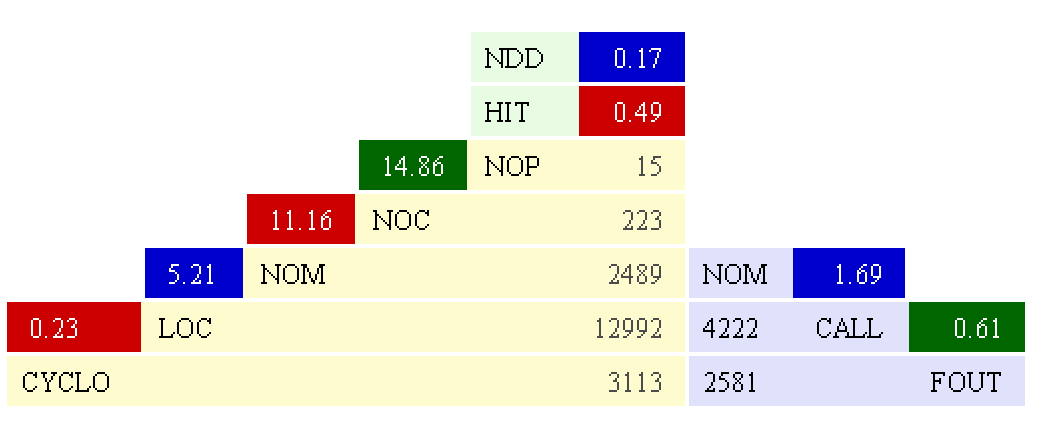
\includegraphics[width=\linewidth]{fig/JHotDraw_iPlasma.png}
  \caption{An overview pyramid of the Java JHotDraw project generated with iPlasma.}
  \label{fig:JHotDraw_iPlasma}
\end{figure}

\begin{figure}[H]
  \centering
  \includesvg[width=\linewidth]{fig/pyramid_SHotDraw.svg}
  \caption{An overview pyramid of the Scala SHotDraw project, generated with Scalade. (Same as figure \ref{fig:pyramid_SHotDraw})}
  \label{fig:pyramid_SHotDraw_Again}
\end{figure}

\subsection{Verifying Cyclomatic Complexity (WMC, CC or CYCLO)}
Although some differences exist between the Scala implementation and the PMD implementation, cyclomatic complexity seems to have likewise results in both implementations. We verified this by calculating the CC of each class in the SHotDraw project with our Scala implementation and calculating the CC for each class in the Java implementation. The results are then plotted, and the correlation is calculated. As \ref{fig:good_WMC_correlation} shows, the correlation is 98\%. Also, here we cannot make strong statements on how alike the 2 implementations perform. However, CC will only be used in places with fuzzy logic, and trust that the CC implementation will fit our needs.
\begin{figure}[H]
    \centering
    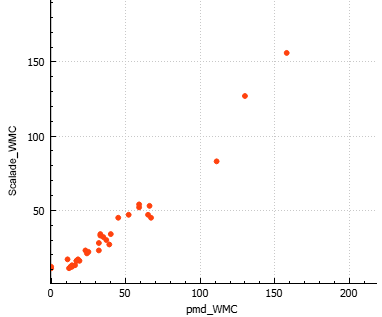
\includegraphics[width=200pt]{fig/good_WMC_correlation.PNG}
    \caption{Both implementations of WMC do correlate with coefficient=98\%}
    \label{fig:good_WMC_correlation}
\end{figure}


\subsection{Comparing the thresholds to Java.} \label{comparing_tresholds}
The iPlasma project can show an overview pyramid for Java projects. The license allows decompiling the project and extracting what values were used to color-grade the metrics in the Overview Pyramid\footnote{\url{https://gitlab.soft.vub.ac.be/maproef1819-emile/maproef1819-emile/blob/master/iPlasma_decompiled/decompiled_result/lrg/insider/plugins/tools/OverviewPyramid.java\#L66}}. This is shown in figure \ref{fig:statistics-iPlasma}. However, these numbers are gained from an unknown selection of projects. Those projects might be selected in a different way than we did in the Scala language, and thus suffer from a different selection bias. To minimize this error, we went through the same selection procedure as we did for Scala projects \ref{running_large_scala_analysis}, but this time for Java projects.

\begin{enumerate}
    \item We downloaded 900 projects from Github using the API. Sorted on number of forks. Only the projects with a 'src' path maximum one folder deep from root where selected.
    \item Only the projects that did compile on the first try where selected.
    \item This brought the project number down to 562 On which we performed the statistics.
    \item After the statistics where calculated, only projects with more than 500LOC where selected, leaving only 259 projects. (List available in appendix \ref{appendix_list_of_analyzed_java_projects})
\end{enumerate}

We used this technique to extract the threshold values that are typical in an open source Java project. Those have been plotted in the same graph over each other \ref{fig:simple_java_scala}. Note that the values differ from the values found for the Scala projects. This could be because of differences in the tools used to calculate these metrics or in, the structural difference between Java and Scala code or the type of projects that are made open source. This difference is not a bad indication, as the thresholds in Scala are re-calculated based its own metrics.
\begin{figure}[H]
    \centering
    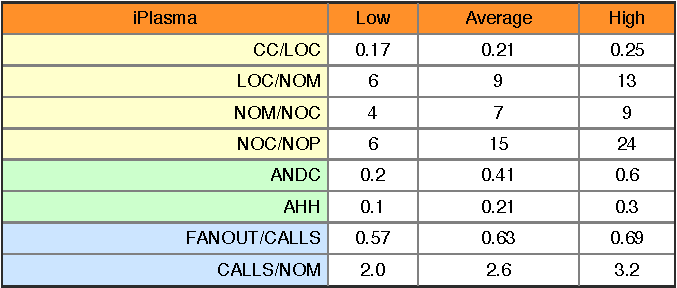
\includegraphics[width=300pt]{fig/statistics-iPlasma.pdf}
    \caption{The results of various ratios taken from the decompiled iPlasma project}
    \label{fig:statistics-iPlasma}
\end{figure}

\begin{figure}[H]
  \centering
  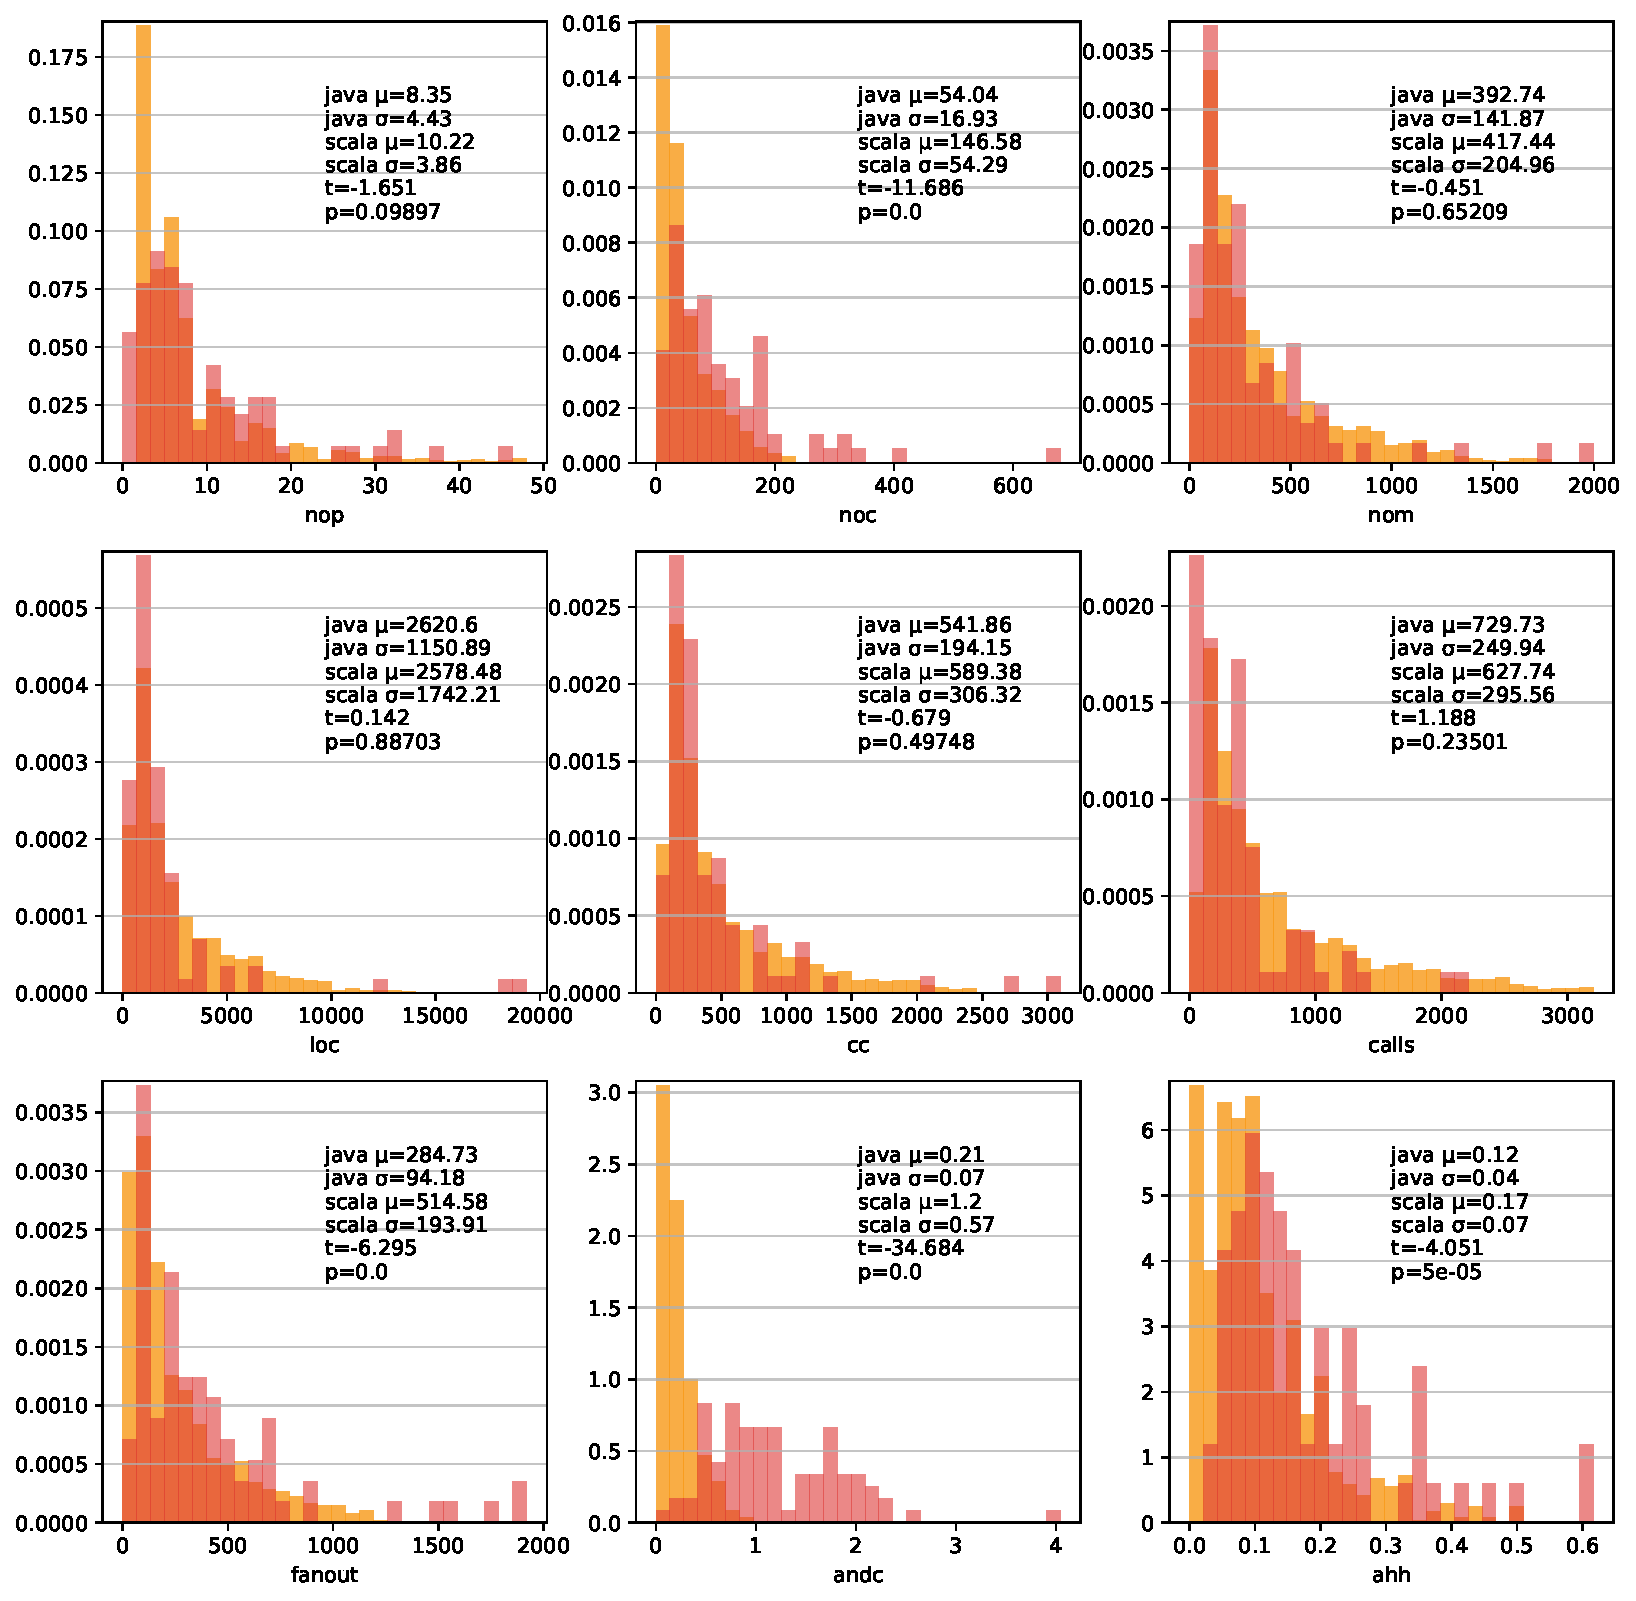
\includegraphics[width = \linewidth]{fig/hist_ratios/simple_java_scala.pdf}
  \caption{A comparison between the metrics between Scala and Java.}
  \label{fig:simple_java_scala}
\end{figure}


Even though the metrics measure very different data, most of them follow similar distributions. 4 out of 9 metrics do however have a different tendance (p<5\%). The difference in the ANDC and AHH metric can probably be explained by how traits in Scala are always taken in the type hierarchy even though they fulfil the function of an interface. As discussed in section \ref{overview_pyramid_AHH}. Considering the language barrier, the overview pyramid of SHotDraw with Scalade shares a lot of properties with the overview pyramid of JHotDraw with iPlasma. As shown in section \ref{section_compare_pyramids}. 


\subsection{Is the last commit always representative for the project?}
For each project we analyze, we only take the last commit. This could be an inaccurate representation of the whole project if there would be large fluctuations between commits. We show that this is no big concern, by analyzing each commit of a project and searching for trends. We discovered that projects tend to have very consistent values for their metrics. If we take the MoVE\footnote{\url{https://github.com/THM-MoTE/MoVE}} project for example, we see that with each commit the ratio between the parameters stays the same. (Figure \ref{fig:graph_move}).

\begin{figure}[H]
    \centering
    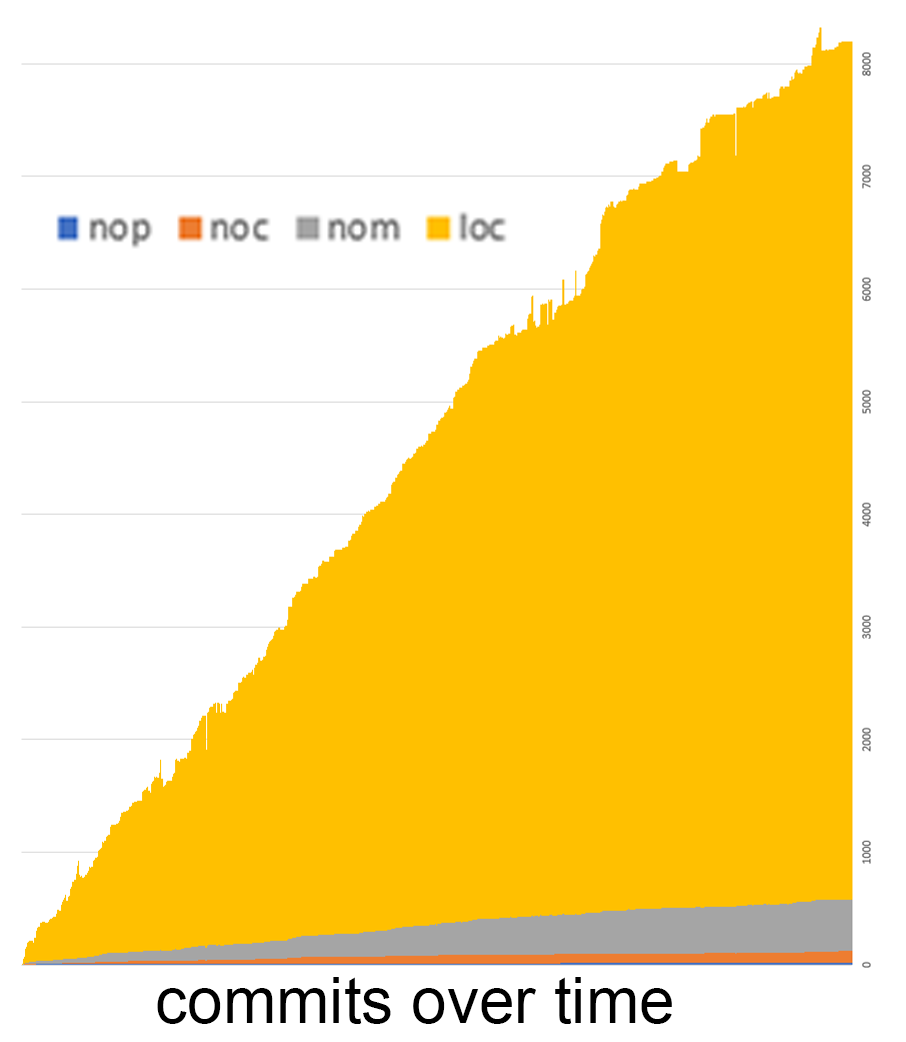
\includegraphics[width=200pt]{fig/graph_move.PNG}
    \caption{Move project's metrics over time}
    \label{fig:graph_move}
\end{figure}


\subsection{Threats to validity}
Re-creating a tool for language makes it difficult to verify if it shows the same exact behavior. However, this poses no problem in the case of the overview pyramid. 
Imagine that one metric, like Cyclomatic Complexity, would structurally give a too small value. The ratio of CYCLO/LOC would structurally be larger than the correct implementation. It won't only be larger in one pyramid, but all of them. We assume that the user of the overview pyramid will mostly look at the color grading of the ratios. If a metric gives offsetted values for each project, the thresholds would be offsetted enough to make sure the color grading still works.


\subsection{GodClass smells against PMD}
As a qualitative verification, we will compare the results of the GodClass smell between SHotDraw with Scalade and JHotDraw with PMD. Both tools generated a list of GodClasses, many classes are common, only 2 extra classes were detected by PMD: Geom and PolygonFigure. 

\textbf{Geom} is a class with only static functions and almost no properties. Pmd detects TCC=0, WMC=53 and ATFD=57, this makes it a GodClass. However, Scalade doesnt detect it, because in Scala, this class is implemented as an Object and those are not considered in Scalade. The same goes for \textbf{PolygonFigure}. PolygonFigure contains many static properties and has been implemented in Scala as a class with a companion, reducing the amount of code in the class and making it not qualify as GodClass.

PMD detects the following GodClasses in the JHotDraw project: The bold classes only appear in PMD and not in Scalade.
\begin{itemize}
    \item AbstractFigure
    \item CompositeFigure
    \item ConnectionTool
    \item DrawApplication
    \item \textbf{Geom}
    \item LineConnection
    \item \textbf{PolygonFigure}
    \item PolyLineFigure
    \item StandardDrawingView
    \item TextFigure
\end{itemize}


\section{Conclusion}

In this thesis, we discussed and implemented multiple ways to automatically asses large Scala software projects. With the overview pyramid, we could generate a quick overview of a Scala project, see how big it is, and how it is structured compared to an average Scala project.

In previous chapter, we evaluated how Scalade performs with a qualitative study. It showed that Scalade can be used to detect real design smells in the code, and that the overview pyramid gives a good idea of the proportions of a project. However, those tools are difficult to verify if they will produce results as their equivalent in Scala. Some metrics have been checked for common patterns in Scala projects and Java project, but no strong conclusions could be made.

All in all, Scalade is a ready to use tool, and has already been used by the author to verify his own Scala projects. We hope that this tool could prove handy for the rest of the Scala community, that's why it is available open source under the MIT license and is ready of anyone to use \footnote{\url{https://github.com/EmileSonneveld/maproef1819-emile}}. 

\subsection{Future work}
\begin{itemize}
    \item An interesting research could be to run the project on many student programming assignments. It could then be possible to verify if there is any correlation between the points of the assignments and the amount of code smells detected.
    \item More design smells could be qualitatively evaluated by Scala experts to gain a better insight of the recall and precision of Scalade.
    \item Many projects were analyzed in this thesis. It could be helpful for the maintainers of those projects to have a website to explore the detected code smells.
    \item Other code smells could be implemented too. Right now, only GodClass, FeatureEnvy and BrainMethod are implemented. But, Tradition Breaker, Refused Parent Bequest, Intensive Coupling, Dispersed Coupling and Shotgun Surgery could be implemented too. See \cite{lanza2007object} for more information.
\end{itemize}

Thank you.

\bibliographystyle{apacite}
\bibliography{thesisEmile.bib}



\section{Appendix}
\subsection{List of analyzed Scala projects} \label{appendix_list_of_analyzed_projects}
241 projects, sorted alphabetically:
100x.io, 99ScalaProblems, abandon, abcdefghppp-google-cloud-22cpu-128GB, after-party, agigaGradableAdjFinder, akka-gameserver, akka-goose-game, akka-http-google-home, akka-http-google-login, akka-playground, akka-raft, akka-sample-cluster-on-google-platform, akka-samples, akka-stream-test, algorithms, appliedfp, ascii-graphs, atmos, atomic-scala-book-excercises, bacala, BatchGeocodingInScalaUsingGoogleAPI, bayes-scala, be\ zug-eventsourcing, BioinformaticsAlgorithmsPart1, blueprints-scala, bus\_driver\_gossip, case-class-\ generator, Catwalk, chess, chisel-tutorial, chisel2-deprecated, codacy-gometalinter, content-deli\ very-system-v4, cosas, cosc455-Gonzalez-lab4, CreateGoogleCourseGroups, CTT-editor, data.go, DieStats, DOS\_Project2\_Gossip\_Simulator, dregex, druthers, escalade-backlog, everythingMust\ Go, fabricator, finagle-postgres, finagle-smtp, FlashFry, fm-flatfile, form-binder, fp-to-the-max, fs2-google-cloud-pubsub, Functional-Go-Fish, functional-google-code-jam, functional\_scala, gaferencer, GameContentSolved, gfc-concurrent, git-hooks-plugin, Go-Fish, go-play-nice, go-tickets, Goals, gobc-transformer, Gobumap-UDC\_ID-Generator, gocardless-scala, gocd-config-cleaner, gocd-dns-poller, GoDataMassager, goedverhaal, gof-design-patterns, GoGame, gokata, gol-gif-bot, GoL-Tp1, gol\_scala, GoldBug, GoldenGateKafkaStreamsConsumer, goldmans-sachs-inter\ view, GoldMiner, GolemSlack, goliath, GoLStrategyGUI, Gomoku, gomovies-crawler, gone-with-the-wind, GoneWithTheWindKiwiPower, good\_companies, goodlord-avanco, GoodsManager, google-action-scala-sdk, google-api-scala, Google-Authenticator, google-cloud-dataflow\ -example, google-cloud-dataflow-example-project, google-cloud-logging, google-cloud-storage-play\ ground, google-directory-lambda-authorizer, google-extractor, google-finance-test, google-finan\ ce-test-work, google-maps-api-ws-scala-client, google-maps-services-scala, google-oauth4s, google-parser-proxy, google-places-api, google-pubsub-alpakka-scala-wrapper, google-pubsub-scala, goo\ gle-safebrowsing2, google-search-archive-parser, google-search-history, Google-Search-History-E\ xplorer, Google-Sign-In-Example, google-storage-sink, google-vision-api, googleapi.scala.js, goog\ leclient, googlecloud-shapeless, GoogleFileOrganizer, googleHash2016, GoogleProtoBuf, GoogleSearch, googlespreadsheet-sample, GoogleTablesUpdate, goos-scala, goos-sniper, goose-game-kata, goose-game-pkupidura, goose-kata, GooseGame, GoScalaScraper, gossip-girl, gossipcala, GossipSim, goticks, goticks-app, goto-cassandra-spark, GoToHack-TestTask, GoToHack2018, goulash, goupil, gov-analytics, graph-goliath, GreekGodsAPI, hayago, hivemq-google-pubsub-plugin, http4s-google-auth, index-builder, inflatable, iservport-google-chart, IsRed, jedi-io, JM\ HC, josimtext, jsengine, JsonGolangStruct, KhanAcademyCSBasics, koauth, lars, learn-scala-the-good-way, Leo-III, LGWM, libanius, liftmodules-googleanalytics, LoMRF, markovGoodness, maxmind-geoip2-scala, MC-Gobang, Model-GameServer-Akka-Streams, mpjsons, nexbook, nlp-research, old-good-prime-numbers, OnGoingPatients, owl-akka-goodies, ozb-google-oauth2-utils, pa-football-client, PackUpdate, pagination-google-scala, PicoGo, play-go, play-googleauth, play-redis, pokemon-go-akka-http, PokemonDnD, pokemonGo, pokermon-go, projectEuler, PushSumAndGossip, qgf, questGo, rainer, rdf-toolkit, red-book, rex, RouletteGo, rpn, RxScala, s\_mach.fsm, saxophone, sbt-google-cloud-storage, scala-akka-self-throttling-prototype, scala-asy\ nc, scala-datatable, scala-debord-gow, scala-go, scala-gol-2015, scala-golang-converter, scala-redis-nb, scala-smtlib, scala-uri, scala99, scaladelray, scalaGoose, ScalaTest, sGoogle, shade, ShExcala, silex, Skene, snowplow-google-cloud-storage-loader, spark-goo\ gle-analytics, spark-google-spreadsheets, spark-streaming-with-google-cloud-example, spark-xml, spray-google-eleva\ tion, subcut, sweet-tooth, sync-godaddy, tap-fp-challenge, testdata, Tinker, traffic-lights-control, UberLogin, vFunk, w, wc-chap2, WolfGoatCabbageProblem, xitrum-google-vision, ZIO-Tests

\subsection{List of analyzed Java projects} \label{appendix_list_of_analyzed_java_projects}
259 projects, sorted alphabetically:
ABAGAIL, activemq, activemq-artemis, Activiti, addressbook-level4, aeron, aima-java, AlgoDS, Algorithms, aliyun-openapi-java-sdk, ambari, android, android-basic-samples, Android-Bootstrap, android-classyshark, Android-CleanArchitecture, android-gpuimage, android-obd-reader, android-saripaar, android-utils, androidannotations, angel, ansj\_seg, antlr4, AnySoftKeyboard, Aria, armeria, arthas, async-http-client, atmosphere, auto, AutoLoadCache, avro, awesome-java-leetcode, aws-doc-sdk-examples, aws-sdk-android-samples, aws-sdk-java, AxonFramework, bc-java, beakerx, beam, bitcoinj, bitlet, blynk-server, BottomBar, brave, buck, BuildCraft, caffeine, calcite, camel, camerakit-android, camunda-bpm-platform, cas, cassandra, cat, cdhproject, cling, cloudstack, codegen, connectbot, Conversations, cordova-android, cordova-plugin-camera-preview, CoreNLP, crawler4j, crunch, ctakes, cuke4duke, curator, curso-java-basico, cxf, cyclops-integration, dagger, DataStructureAndAlgorithmsMadeEasyInJava, dbeaver, deepdsl, DeepLearning, deeplearning4j, dex2jar, dialogplus, digitalocean-api-java, DiskLruCache, docker-client, docker-maven-plugin, docx4j, drill, drools, dropwizard, dsl-json, DSpace, dubbo, e-commerce-rest-api, easyexcel, EasyReport, effective-java-examples, elasticsearch, elasticsearch-analysis-ik, EventBus, ExoPlayer, fabric-sdk-java, fastdfs-client-java, feign, ffmpeg-android-java, find-sec-bugs, flink, flume, flyingsaucer, flyway, fnlp, ForestBlog, framework, freedomotic, funiture, gecco, geoserver, geotools, getting-started-java, github-api, glide-transformations, gnucash-android, google-api-java-client, google-api-java-client-samples, google-cloud-java, google-java-format, google-maps-services-java, gpmall, gpslogger, graal, gradle-retrolambda, graphhopper, greys-anatomy, groovy, grpc-java, gson, guice, h2o-3, hapi-fhir, hawtdispatch, hawtio, hazelcast, hbase, heritrix3, hibernate-orm, HikariCP, hive, hsweb-framework, http-request, huaweicloud-cs-sdk, hutool, idea-sbt-plugin, ip2region, itchat4j, j2objc, jacoco, jadx, java-8-lambdas-exercises, java-algorithms-implementation, java-apns, java-cas-client, java-client, java-concurrent-hash-trie-map, java-core-learning-example, java-design-patterns, java-docs-samples, java-driver, java-game-server, java-jwt, java-learning, java-sdk, Java-WebSocket, java\_practical\_semantic\_web, javacpp-presets, javamelody, JavaMultiThreading, javaparser, javapoet, JavaWEB, JAViewer, JCSprout, jd-gui, jeecg-boot, jena, jenkins, Jest, jetcache, jetty.project, JFoenix, jhipster-sample-app, jib, jieba-analysis, jjwt, jmeter, jmonkeyengine, jna, jodd, journaldev, JsonPath, jsonschema2pojo, junit5, Jupiter, jutils, jwt-spring-security-demo, kafka, karaf, killbill, kubernetes-client, lanproxy, LeetCode-Sol-Res, libgdx, libstreaming, light-task-scheduler, line-bot-sdk-java, logback, Luyten, mage, mahout, mall, mapdb, marytts, material, material-calendarview, material-menu, material-ripple, materialistic, MaterialViewPager, maven, Memcached-Java-Client, metrics, micronaut-core, mysql-binlog-connector-java, netty-socketio, NettyRPC, oauth2play2scala, opslabJutil, PayMap, pig, pybbs, red5-server, reflections, scala-maven-plugin, scalagwt-sample, scalardb, ScalaShade, SHotDraw, socket.io-client-java, solo, sonar-scala, sonar-scala-plugin, spark, spring-data-elasticsearch, stream-lib, symphony, thumbnailator, transmittable-thread-local, WebCollector, wechat4j, word, ysoserial


\subsection{Results of detected design smells in the sample projects} \label{appendix_design_smells_in_sample_projects}
The 241 selected Scala projects where analyzed for design smells, and these are the results:

 \begin{tabular}{|c c c|} 
 \hline
 project & construct name & smell \\ [0.5ex] 
 \hline\hline
Leo-III & SchedulerImpl\#SchedulerRun\#run(). & FeatureEnvy \\
Leo-III & SchedulerImpl\#GenFilter\#run(). & FeatureEnvy \\
Leo-III & SchedulingAgent\#filter(). & FeatureEnvy \\
Leo-III & BoolextRule\#BoolextHint\#apply(). & FeatureEnvy \\
Leo-III & CNFRule\#CNFHint\#apply(). & FeatureEnvy \\
Leo-III & FuncExtRule\#FuncExtHint\#apply(). & FeatureEnvy \\
Leo-III & LiftEqRule\#LiftEqHint\#apply(). & FeatureEnvy \\
Leo-III & SubsumptionRule\#MovingSubsumptionHint\#apply(). & FeatureEnvy \\
Leo-III & UnificationRule\#UnificationHint\#apply(). & FeatureEnvy \\
Leo-III & HOMatching.EnumUnifier\#apply(). & FeatureEnvy \\
Leo-III & HuetsPreUnification.EnumUnifier\#apply(). & FeatureEnvy \\
Leo-III & LambdaElim\_SKI\#eliminateLambdaNewShallow(). & FeatureEnvy \\
Leo-III & LambdaElim\_SKI\#eliminateLambdaNew0(). & FeatureEnvy \\
Leo-III & GeneralStateImp\# & GodClass \\
Leo-III & STIndex\#addClause(). & FeatureEnvy \\
Leo-III & DelayedUnificationAgent\#DelayedUnificationTask\#run(). & FeatureEnvy \\
Leo-III & ExternalAgent\#ExtResultTask\#run(). & FeatureEnvy \\
Leo-III & InterleavingLoop\#mainLoopInferences(). & FeatureEnvy \\
Leo-III & InterleavingLoop\#apply(). & BrainMethod \\
CTT-editor & CrudServer.StaticHandler\#handle(). & BrainMethod \\
scalameta & ExploreMacros\# & GodClass \\
dregex & RegexParser\# & GodClass \\
FlashFry & GenerateRandomFasta\#run(). & FeatureEnvy \\
FlashFry & BedAnnotation\#scoreGuides(). & FeatureEnvy \\
FlashFry & DangerousSequences\#scoreGuide(). & FeatureEnvy \\
GameContentSolved & Datafier.TranslationContext\#FieldTranslation.toData(). & FeatureEnvy \\
GameContentSolved & package.RichValueType\#asData(). & FeatureEnvy \\
GameContentSolved & package.RichRefType\#asData(). & FeatureEnvy \\
GameContentSolved & package.RichSelectOneType\#asData(). & FeatureEnvy \\
GameContentSolved & package.RichField\#asData(). & FeatureEnvy \\
GameContentSolved & ResourceLibrary\# & GodClass \\
GameContentSolved & SchemaPage\#getChildren(). & FeatureEnvy \\
GameContentSolved & ListAndEditScreen\#makeViewItem(). & FeatureEnvy \\
google-safebrowsing2 & SafeBrowsing2\#lookup\_hostKey(). & FeatureEnvy \\
 \hline
 \end{tabular}
 \newpage
 \begin{tabular}{|c c c|} 
 \hline
 project & construct name & smell \\ [0.5ex] 
 \hline\hline
LoMRF & LogicOps.DefiniteClausesOps\#collectAndMerge(). & FeatureEnvy \\
LoMRF & KBParser\# & GodClass \\
LoMRF & KBParser\#normaliseVariableDomains(). & FeatureEnvy \\
LoMRF & KBParser\#atomicFormulaPrefix(). & FeatureEnvy \\
LoMRF & ClauseGrounderImpl\#substituteTerm(). & FeatureEnvy \\
LoMRF & ClauseLiteralsOrdering\#compare(). & FeatureEnvy \\
LoMRF & MaxWalkSAT\#infer(+1). & FeatureEnvy \\
LoMRF & MCSAT\#infer(). & FeatureEnvy \\
LoMRF & MCSAT\#infer(). & BrainMethod \\
LoMRF & HyperGraph\#findPaths(+1). & FeatureEnvy \\
LoMRF & PlaceMarker\#toString(). & BrainMethod \\
LoMRF & OSL\#reviseTheory(). & FeatureEnvy \\
LoMRF & SupervisionGraph\#solve(). & FeatureEnvy \\
LoMRF & MaxMarginLearner\#writeResults(). & FeatureEnvy \\
LoMRF & OnlineLearner\#writeResults(). & FeatureEnvy \\
LoMRF & AtomEvidenceDBBuilder\#`+=`(). & FeatureEnvy \\
LoMRF & EvidenceBuilder\#DefaultFunctionRegister\#insert(). & FeatureEnvy \\
LoMRF & EvidenceBuilder\#FunctionToAUXPredRegister\#insert(). & FeatureEnvy \\
LoMRF & MRFState\# & GodClass \\
LoMRF & MRFState\#flip(). & FeatureEnvy \\
w & Slide\# & GodClass \\
w & WLabelSkin\# & GodClass \\
s\_mach.fsm & package.TransitionAccumulator\#accumulate(). & FeatureEnvy \\
scaladelray & Plane\#`<--`(). & FeatureEnvy \\
scaladelray & LambertMaterial\#colorFor(). & FeatureEnvy \\
scaladelray & LightBlendingMaterial\#colorFor(). & FeatureEnvy \\
scaladelray & TransparentMaterial\#colorFor(). & FeatureEnvy \\
scaladelray & ModelProvider\# & GodClass \\
scala-redis-nb & PipelineStage\#`>>`(). & FeatureEnvy \\
scala-redis-nb & RedisConnection\#unconnected(). & FeatureEnvy \\
bacala & Version\#compare(). & BrainMethod \\
bacala & IDescriptor\#filterArtifacts(). & FeatureEnvy \\
nexbook & DbUpdateOrderChangeHandler\#onOrderFillChange(). & FeatureEnvy \\
nexbook & ResultLogger\#logResultToFile(). & FeatureEnvy \\
abandon & RegisterReportSettings\#groupOp(). & FeatureEnvy \\
abandon & AccountState\#updateAmounts(). & FeatureEnvy \\
ascii-graphs & Layouter\#spaceVertices(+1). & FeatureEnvy \\
ascii-graphs & Layouter\#makeEdgeInfos(). & FeatureEnvy \\
ascii-graphs & Renderer\# & GodClass \\
ascii-graphs & Renderer\#render(+2). & FeatureEnvy \\
ascii-graphs & QuadTree\#quadrate(+1). & FeatureEnvy \\
atmos & LogEventsWithSlf4j\#isLoggable(). & FeatureEnvy \\
bayes-scala & LoopyBP\#calibrateCluster(). & FeatureEnvy \\
bayes-scala & LoopyBP\#isCalibrated(). & FeatureEnvy \\
bayes-scala & LoopyBP\#clusterBelief(). & FeatureEnvy \\
bayes-scala & LoopyBP\#logLikelihood(). & FeatureEnvy \\
bayes-scala & LoopyBP\#marginal(). & FeatureEnvy \\
bayes-scala & LoopyBP\#setEvidence(). & FeatureEnvy \\
bayes-scala & GenericEP\#marginal(). & FeatureEnvy \\
case-class-generator & Constructor\#dump(). & FeatureEnvy \\
case-class-generator & CopyDefault\#dump(). & FeatureEnvy \\
case-class-generator & Equals\#dump(). & FeatureEnvy \\
case-class-generator & Init\#dump(). & FeatureEnvy \\
case-class-generator & ModuleApply\#dump(). & FeatureEnvy \\
case-class-generator & ModuleUnapply\#dump(). & FeatureEnvy \\
 \hline
 \end{tabular}
 \newpage
 \begin{tabular}{|c c c|} 
 \hline
 project & construct name & smell \\ [0.5ex] 
 \hline\hline
chisel2-deprecated & Backend\# & GodClass \\
chisel2-deprecated & Backend\#sortComponents(). & FeatureEnvy \\
chisel2-deprecated & Backend\#nameAll(). & FeatureEnvy \\
chisel2-deprecated & Backend\#renameNodes(). & FeatureEnvy \\
chisel2-deprecated & Backend\#assignClockAndResetToModules(). & FeatureEnvy \\
chisel2-deprecated & Backend\#addClocksAndResets(). & FeatureEnvy \\
chisel2-deprecated & Backend\#gatherClocksAndResets(). & FeatureEnvy \\
chisel2-deprecated & Backend\#nameRsts(). & FeatureEnvy \\
chisel2-deprecated & Backend\#createClkDomain(). & FeatureEnvy \\
chisel2-deprecated & Backend\#addBindings(). & FeatureEnvy \\
chisel2-deprecated & Backend\#findCombLoop(). & FeatureEnvy \\
chisel2-deprecated & Backend\#W0Wtransform(). & FeatureEnvy \\
chisel2-deprecated & CppBackend\# & GodClass \\
chisel2-deprecated & CppBackend\#emitInit(). & FeatureEnvy \\
chisel2-deprecated & DotBackend\# & GodClass \\
chisel2-deprecated & FloBackend\#emit(). & BrainMethod \\
chisel2-deprecated & Module\# & GodClass \\
chisel2-deprecated & Node\# & GodClass \\
chisel2-deprecated & Op\#review(). & BrainMethod \\
chisel2-deprecated & Tester\# & GodClass \\
chisel2-deprecated & VcdBackend\# & GodClass \\
chisel2-deprecated & VerilogBackend\# & GodClass \\
chisel2-deprecated & VerilogBackend\#emitPortDef(). & FeatureEnvy \\
chisel2-deprecated & VerilogBackend\#emitDec(). & FeatureEnvy \\
chisel2-deprecated & VerilogBackend\#emitRegs(). & FeatureEnvy \\
chisel2-deprecated & ArbiterSuite\#testArbiter(). & FeatureEnvy \\
chisel2-deprecated & ArbiterSuite\#testStableArbiter(). & FeatureEnvy \\
chisel2-deprecated & ArbiterSuite\#testDefaultLockingArbiter(). & FeatureEnvy \\
chisel2-deprecated & ArbiterSuite\#testDefaultStableLockingArbiter(). & FeatureEnvy \\
chisel2-deprecated & ArbiterSuite\#testLockingArbiter(). & FeatureEnvy \\
chisel2-deprecated & ArbiterSuite\#testStableLockingArbiter(). & FeatureEnvy \\
chisel2-deprecated & ArbiterSuite\#testRRArbiter(). & FeatureEnvy \\
chisel2-deprecated & ArbiterSuite\#testStableRRArbiter(). & FeatureEnvy \\
chisel2-deprecated & ArbiterSuite\#testDefaultRRLockingArbiter(). & FeatureEnvy \\
chisel2-deprecated & ArbiterSuite\#testDefaultStableRRLockingArbiter(). & FeatureEnvy \\
chisel2-deprecated & ArbiterSuite\#testRRLockingArbiter(). & FeatureEnvy \\
chisel2-deprecated & ArbiterSuite\#testStableRRLockingArbiter(). & FeatureEnvy \\
chisel2-deprecated & ConnectSuite\#testResetConnections(). & FeatureEnvy \\
chisel2-deprecated & VerifSuite\#AssertTesterCommon\#queue(). & FeatureEnvy \\
chisel2-deprecated & VerilogMultiModule\#testVerilogMultiModule(). & FeatureEnvy \\
 \hline
 \end{tabular}
 \newpage
 \begin{tabular}{|c c c|} 
 \hline
 project & construct name & smell \\ [0.5ex] 
 \hline\hline
druthers & OptionsParser\# & GodClass \\
druthers & OptionsParser\#Parse\#consumeSpec(+1). & FeatureEnvy \\
fabricator & CsvFileBuilder\# & GodClass \\
fabricator & DateRange\#getRangeList(). & FeatureEnvy \\
fabricator & FileGenerator\#fileExtension(+1). & FeatureEnvy \\
fabricator & FileGenerator\#mime\_type(+1). & FeatureEnvy \\
fabricator & AlphaNumericTestSuite\# & GodClass \\
fabricator & CalendarTestSuite\# & GodClass \\
fabricator & CalendarTestSuite\#dateFormats(). & FeatureEnvy \\
fabricator & CalendarTestSuite\#datesRangeDP(). & FeatureEnvy \\
fabricator & ContactTestSuite\# & GodClass \\
fabricator & ContactTestSuite\#birthdayWithFormatsDP(). & FeatureEnvy \\
fabricator & FileTestSuite\#testCustomCsv(). & FeatureEnvy \\
fabricator & FileTestSuite\#fileTypeDP(). & FeatureEnvy \\
fabricator & FileTestSuite\#mimeTypeDP(). & FeatureEnvy \\
fabricator & FinanceTestSuite\# & GodClass \\
fabricator & InternetTestSuite\#testUrlAsUri(). & FeatureEnvy \\
finagle-postgres & BackendMessageParser\# & GodClass \\
fm-flatfile & RichXMLStreamReader2\# & GodClass \\
jedi-io & EtagCacheConfig\#cacheFor(). & FeatureEnvy \\
jedi-io & TimeSensitiveEtagCachedEntry\#cacheFor(). & FeatureEnvy \\
jedi-io & UrlLocation\#createRequester(). & FeatureEnvy \\
mpjsons & DeserializerFactoryImpl\# & GodClass \\
mpjsons & DeserializerFactoryImpl\#getPureDeserializerNoCache(). & BrainMethod \\
mpjsons & SerializerFactoryImpl\#getSerializerNoCache(). & BrainMethod \\
RxScala & RxScalaDemo\# & GodClass \\
RxScala & ObservableTests\# & GodClass \\
scala-smtlib & SemanticsDriver\# & GodClass \\
scala-smtlib & ProcessInterpreter\#parseResponseOf(). & FeatureEnvy \\
scala-smtlib & PrintingContext\# & GodClass \\
scala-smtlib & PrintingContext\#print(). & FeatureEnvy \\
scala-smtlib & PrintingContext\#printCommand(). & FeatureEnvy \\
scala-smtlib & PrinterTests\# & GodClass \\
scala-smtlib & PrinterTests\#testCommandsResponses(). & FeatureEnvy \\
ScalaTest & IndexedColorFilter\#indexedImage(). & FeatureEnvy \\
ScalaTest & BarnesHut.BarnesHutFrame\#stepThroughSimulation(). & FeatureEnvy \\
ScalaTest & SimulationCanvas\#paintComponent(). & FeatureEnvy \\
ScalaTest & Simulator\#updateBoundaries(). & FeatureEnvy \\
ScalaTest & Simulator\#mergeBoundaries(). & FeatureEnvy \\
ScalaTest & BloxorzSuite\#SolutionChecker\#solve(). & FeatureEnvy \\
ShExcala & ShExDoc\# & GodClass \\
vFunk & IPv6\#getErrors(). & BrainMethod \\
good\_companies & CloudClient\#makeParent(). & FeatureEnvy \\
good\_companies & CloudClient\#makeChild(). & FeatureEnvy \\
google-cloud-logging & LoggingAppender\# & GodClass \\
 \hline
 \end{tabular}
 \newpage
 \begin{tabular}{|c c c|} 
 \hline
 project & construct name & smell \\ [0.5ex] 
 \hline\hline
goose-game-kata & GameEvent\#logic(). & FeatureEnvy \\
goose-game-kata & GooseGame\#applyRoll(). & FeatureEnvy \\
gossipcala & ResultAnalyser\#analyse(). & FeatureEnvy \\
PackUpdate & Update.NewComponent\#runDownload(). & FeatureEnvy \\
PackUpdate & InstalledComponent\#validateIntegrity(). & FeatureEnvy \\
RouletteGo & gui\#redraw(). & FeatureEnvy \\
RouletteGo & controller\#Step(). & FeatureEnvy \\
RouletteGo & Solver\#checkforWin(). & FeatureEnvy \\
spark-google-analytics & AnalyticsRelation\# & GodClass \\
spark-xml & DomXmlParser\#readChildNodes(). & FeatureEnvy \\
cafebabe & CodeHandler\#computeMaxStack(). & FeatureEnvy \\
chisel3 & Data\# & GodClass \\
chisel3 & BaseModule\#\_bindIoInPlace(). & FeatureEnvy \\
chisel3 & InjectingAspect\#toAnnotation(+1). & FeatureEnvy \\
chisel3 & Emitter\#moduleDefn(). & FeatureEnvy \\
dbstress & ControllerActor\#receive(). & FeatureEnvy \\
dbstress & DatabaseActor\#receive(). & FeatureEnvy \\
dice\_poker\_software\_engineering & Tui\#update(). & FeatureEnvy \\
dice\_poker\_software\_engineering & DPController\# & GodClass \\
dice\_poker\_software\_engineering & DPController\#higherBidIsNotPossible(). & FeatureEnvy \\
akka-server & PipelineStage\#`>>`(). & FeatureEnvy \\
akka-server & StorageService\#handleAuth(). & FeatureEnvy \\
akka-server & Room\#getPoint(). & FeatureEnvy \\
SHotDraw & DrawApplication\# & GodClass \\
SHotDraw & JHDDropTargetListener\#drop(). & BrainMethod \\
SHotDraw & ElbowHandle\#constrainX(). & FeatureEnvy \\
SHotDraw & ElbowHandle\#constrainY(). & FeatureEnvy \\
SHotDraw & LineConnection\# & GodClass \\
SHotDraw & PolyLineFigure\# & GodClass \\
SHotDraw & TextFigure\# & GodClass \\
SHotDraw & AbstractFigure\# & GodClass \\
SHotDraw & CompositeFigure\# & GodClass \\
SHotDraw & ConnectionTool\# & GodClass \\
SHotDraw & StandardDrawingView\# & GodClass \\
SHotDraw & StandardDrawingView\#insertFigures(). & FeatureEnvy \\
SHotDraw & RedoCommand\#execute(). & FeatureEnvy \\
SHotDraw & UndoCommand\#execute(). & FeatureEnvy \\
 \hline
 \end{tabular}
 

\end{document}
